% Options for packages loaded elsewhere
\PassOptionsToPackage{unicode}{hyperref}
\PassOptionsToPackage{hyphens}{url}
\PassOptionsToPackage{dvipsnames,svgnames,x11names}{xcolor}
%
\documentclass[
  letterpaper,
  DIV=11,
  numbers=noendperiod]{scrartcl}

\usepackage{amsmath,amssymb}
\usepackage{iftex}
\ifPDFTeX
  \usepackage[T1]{fontenc}
  \usepackage[utf8]{inputenc}
  \usepackage{textcomp} % provide euro and other symbols
\else % if luatex or xetex
  \usepackage{unicode-math}
  \defaultfontfeatures{Scale=MatchLowercase}
  \defaultfontfeatures[\rmfamily]{Ligatures=TeX,Scale=1}
\fi
\usepackage{lmodern}
\ifPDFTeX\else  
    % xetex/luatex font selection
\fi
% Use upquote if available, for straight quotes in verbatim environments
\IfFileExists{upquote.sty}{\usepackage{upquote}}{}
\IfFileExists{microtype.sty}{% use microtype if available
  \usepackage[]{microtype}
  \UseMicrotypeSet[protrusion]{basicmath} % disable protrusion for tt fonts
}{}
\makeatletter
\@ifundefined{KOMAClassName}{% if non-KOMA class
  \IfFileExists{parskip.sty}{%
    \usepackage{parskip}
  }{% else
    \setlength{\parindent}{0pt}
    \setlength{\parskip}{6pt plus 2pt minus 1pt}}
}{% if KOMA class
  \KOMAoptions{parskip=half}}
\makeatother
\usepackage{xcolor}
\setlength{\emergencystretch}{3em} % prevent overfull lines
\setcounter{secnumdepth}{5}
% Make \paragraph and \subparagraph free-standing
\makeatletter
\ifx\paragraph\undefined\else
  \let\oldparagraph\paragraph
  \renewcommand{\paragraph}{
    \@ifstar
      \xxxParagraphStar
      \xxxParagraphNoStar
  }
  \newcommand{\xxxParagraphStar}[1]{\oldparagraph*{#1}\mbox{}}
  \newcommand{\xxxParagraphNoStar}[1]{\oldparagraph{#1}\mbox{}}
\fi
\ifx\subparagraph\undefined\else
  \let\oldsubparagraph\subparagraph
  \renewcommand{\subparagraph}{
    \@ifstar
      \xxxSubParagraphStar
      \xxxSubParagraphNoStar
  }
  \newcommand{\xxxSubParagraphStar}[1]{\oldsubparagraph*{#1}\mbox{}}
  \newcommand{\xxxSubParagraphNoStar}[1]{\oldsubparagraph{#1}\mbox{}}
\fi
\makeatother


\providecommand{\tightlist}{%
  \setlength{\itemsep}{0pt}\setlength{\parskip}{0pt}}\usepackage{longtable,booktabs,array}
\usepackage{calc} % for calculating minipage widths
% Correct order of tables after \paragraph or \subparagraph
\usepackage{etoolbox}
\makeatletter
\patchcmd\longtable{\par}{\if@noskipsec\mbox{}\fi\par}{}{}
\makeatother
% Allow footnotes in longtable head/foot
\IfFileExists{footnotehyper.sty}{\usepackage{footnotehyper}}{\usepackage{footnote}}
\makesavenoteenv{longtable}
\usepackage{graphicx}
\makeatletter
\newsavebox\pandoc@box
\newcommand*\pandocbounded[1]{% scales image to fit in text height/width
  \sbox\pandoc@box{#1}%
  \Gscale@div\@tempa{\textheight}{\dimexpr\ht\pandoc@box+\dp\pandoc@box\relax}%
  \Gscale@div\@tempb{\linewidth}{\wd\pandoc@box}%
  \ifdim\@tempb\p@<\@tempa\p@\let\@tempa\@tempb\fi% select the smaller of both
  \ifdim\@tempa\p@<\p@\scalebox{\@tempa}{\usebox\pandoc@box}%
  \else\usebox{\pandoc@box}%
  \fi%
}
% Set default figure placement to htbp
\def\fps@figure{htbp}
\makeatother

\usepackage{fontspec}
\usepackage{multirow}
\usepackage{multicol}
\usepackage{colortbl}
\usepackage{hhline}
\newlength\Oldarrayrulewidth
\newlength\Oldtabcolsep
\usepackage{longtable}
\usepackage{array}
\usepackage{hyperref}
\usepackage{float}
\usepackage{wrapfig}
\usepackage{booktabs}
\usepackage{caption}
\usepackage{anyfontsize}
\KOMAoption{captions}{tableheading}
\makeatletter
\@ifpackageloaded{caption}{}{\usepackage{caption}}
\AtBeginDocument{%
\ifdefined\contentsname
  \renewcommand*\contentsname{Table of contents}
\else
  \newcommand\contentsname{Table of contents}
\fi
\ifdefined\listfigurename
  \renewcommand*\listfigurename{List of Figures}
\else
  \newcommand\listfigurename{List of Figures}
\fi
\ifdefined\listtablename
  \renewcommand*\listtablename{List of Tables}
\else
  \newcommand\listtablename{List of Tables}
\fi
\ifdefined\figurename
  \renewcommand*\figurename{Figure}
\else
  \newcommand\figurename{Figure}
\fi
\ifdefined\tablename
  \renewcommand*\tablename{Table}
\else
  \newcommand\tablename{Table}
\fi
}
\@ifpackageloaded{float}{}{\usepackage{float}}
\floatstyle{ruled}
\@ifundefined{c@chapter}{\newfloat{codelisting}{h}{lop}}{\newfloat{codelisting}{h}{lop}[chapter]}
\floatname{codelisting}{Listing}
\newcommand*\listoflistings{\listof{codelisting}{List of Listings}}
\makeatother
\makeatletter
\makeatother
\makeatletter
\@ifpackageloaded{caption}{}{\usepackage{caption}}
\@ifpackageloaded{subcaption}{}{\usepackage{subcaption}}
\makeatother

\usepackage{bookmark}

\IfFileExists{xurl.sty}{\usepackage{xurl}}{} % add URL line breaks if available
\urlstyle{same} % disable monospaced font for URLs
\hypersetup{
  pdftitle={Utano Market Survey Report},
  pdfauthor={UlwaziHub},
  colorlinks=true,
  linkcolor={blue},
  filecolor={Maroon},
  citecolor={Blue},
  urlcolor={Blue},
  pdfcreator={LaTeX via pandoc}}


\title{Utano Market Survey Report}
\author{UlwaziHub}
\date{}

\begin{document}
\maketitle

\renewcommand*\contentsname{Table of Contents}
{
\hypersetup{linkcolor=}
\setcounter{tocdepth}{3}
\tableofcontents
}

\section{Introduction}\label{introduction}

This report presents the latest findings from the Utano Market Survey,
conducted by UlwaziHUB Consulting Services in South Africa. The survey,
which targeted a diverse population, was administered online between May
30 and June 5. A total of 391 responses were recorded. However 384 have
been considered as valid records while 3 are responses from participants
that did not give consent to the survey. The remaining 3 have been
considered as missing values. Thus, the achieved response rate is
99.7\%. The respondents providing valuable insights into current market
trends, healthcare access, and service preferences. The data collected
serves as a critical foundation for understanding the needs and
expectations of communities, and will inform the design and delivery of
more inclusive and responsive health-related services.

\section{Methods}\label{methods}

The Utano Market Survey employed a cross-sectional study design and was
conducted entirely online using a structured digital questionnaire. The
survey instrument was developed in English and translated into
additional local languages to improve accessibility and comprehension. A
combination of purposive and snowball sampling techniques was used to
recruit participants through social media platforms, community networks,
and digital outreach by local partners.

The questionnaire included both closed- and open-ended questions
covering themes such as demographics, health-seeking behavior, service
delivery preferences, and perceived barriers to healthcare. Data
collection was anonymous, and participants provided informed consent
electronically before beginning the survey. All data were securely
stored and analyzed using statistical software to produce descriptive
and inferential insights, including cross-tabulations and chi-square
tests for associations between key variables such as gender and
nationality.

\section{Results}\label{results}

\section{Section A: Demographic Characteristic of the
Respondents}\label{section-a-demographic-characteristic-of-the-respondents}

This section presents the demographics and distribution of the results

The sampled respondents were from 16 nationalities with 193 (50.1 \%) of
them being females and the remaining 185 (48.1 \%) being males. Table
@@@@ shows a breakdown of the nationalities that responded by gender.

\begin{verbatim}
                    Table 1: Distribution of Males and Females by Country
\end{verbatim}

\global\setlength{\Oldarrayrulewidth}{\arrayrulewidth}

\global\setlength{\Oldtabcolsep}{\tabcolsep}

\setlength{\tabcolsep}{2pt}

\renewcommand*{\arraystretch}{1.5}



\providecommand{\ascline}[3]{\noalign{\global\arrayrulewidth #1}\arrayrulecolor[HTML]{#2}\cline{#3}}

\begin{longtable*}[c]{|p{1.38in}|p{1.20in}|p{1.03in}}



\ascline{1.5pt}{666666}{1-3}

\multicolumn{1}{>{\raggedright}m{\dimexpr 1.38in+0\tabcolsep}}{\textcolor[HTML]{000000}{\fontsize{11}{11}\selectfont{\global\setmainfont{Arial}{Nationality}}}} & \multicolumn{1}{>{\raggedright}m{\dimexpr 1.2in+0\tabcolsep}}{\textcolor[HTML]{000000}{\fontsize{11}{11}\selectfont{\global\setmainfont{Arial}{Female\ (n\ \%)}}}} & \multicolumn{1}{>{\raggedright}m{\dimexpr 1.03in+0\tabcolsep}}{\textcolor[HTML]{000000}{\fontsize{11}{11}\selectfont{\global\setmainfont{Arial}{Male\ (n\ \%)}}}} \\

\ascline{1.5pt}{666666}{1-3}\endfirsthead 

\ascline{1.5pt}{666666}{1-3}

\multicolumn{1}{>{\raggedright}m{\dimexpr 1.38in+0\tabcolsep}}{\textcolor[HTML]{000000}{\fontsize{11}{11}\selectfont{\global\setmainfont{Arial}{Nationality}}}} & \multicolumn{1}{>{\raggedright}m{\dimexpr 1.2in+0\tabcolsep}}{\textcolor[HTML]{000000}{\fontsize{11}{11}\selectfont{\global\setmainfont{Arial}{Female\ (n\ \%)}}}} & \multicolumn{1}{>{\raggedright}m{\dimexpr 1.03in+0\tabcolsep}}{\textcolor[HTML]{000000}{\fontsize{11}{11}\selectfont{\global\setmainfont{Arial}{Male\ (n\ \%)}}}} \\

\ascline{1.5pt}{666666}{1-3}\endhead



\multicolumn{1}{>{\raggedright}m{\dimexpr 1.38in+0\tabcolsep}}{\textcolor[HTML]{000000}{\fontsize{11}{11}\selectfont{\global\setmainfont{Arial}{Zimbabwe}}}} & \multicolumn{1}{>{\raggedright}m{\dimexpr 1.2in+0\tabcolsep}}{\textcolor[HTML]{000000}{\fontsize{11}{11}\selectfont{\global\setmainfont{Arial}{95\ \ (60\%)}}}} & \multicolumn{1}{>{\raggedright}m{\dimexpr 1.03in+0\tabcolsep}}{\textcolor[HTML]{000000}{\fontsize{11}{11}\selectfont{\global\setmainfont{Arial}{63\ \ (40\%)}}}} \\





\multicolumn{1}{>{\raggedright}m{\dimexpr 1.38in+0\tabcolsep}}{\textcolor[HTML]{000000}{\fontsize{11}{11}\selectfont{\global\setmainfont{Arial}{Mozambique}}}} & \multicolumn{1}{>{\raggedright}m{\dimexpr 1.2in+0\tabcolsep}}{\textcolor[HTML]{000000}{\fontsize{11}{11}\selectfont{\global\setmainfont{Arial}{26\ \ (30\%)}}}} & \multicolumn{1}{>{\raggedright}m{\dimexpr 1.03in+0\tabcolsep}}{\textcolor[HTML]{000000}{\fontsize{11}{11}\selectfont{\global\setmainfont{Arial}{60\ \ (70\%)}}}} \\





\multicolumn{1}{>{\raggedright}m{\dimexpr 1.38in+0\tabcolsep}}{\textcolor[HTML]{000000}{\fontsize{11}{11}\selectfont{\global\setmainfont{Arial}{Lesotho}}}} & \multicolumn{1}{>{\raggedright}m{\dimexpr 1.2in+0\tabcolsep}}{\textcolor[HTML]{000000}{\fontsize{11}{11}\selectfont{\global\setmainfont{Arial}{25\ \ (52\%)}}}} & \multicolumn{1}{>{\raggedright}m{\dimexpr 1.03in+0\tabcolsep}}{\textcolor[HTML]{000000}{\fontsize{11}{11}\selectfont{\global\setmainfont{Arial}{23\ \ (48\%)}}}} \\





\multicolumn{1}{>{\raggedright}m{\dimexpr 1.38in+0\tabcolsep}}{\textcolor[HTML]{000000}{\fontsize{11}{11}\selectfont{\global\setmainfont{Arial}{South\ africa}}}} & \multicolumn{1}{>{\raggedright}m{\dimexpr 1.2in+0\tabcolsep}}{\textcolor[HTML]{000000}{\fontsize{11}{11}\selectfont{\global\setmainfont{Arial}{24\ \ (55\%)}}}} & \multicolumn{1}{>{\raggedright}m{\dimexpr 1.03in+0\tabcolsep}}{\textcolor[HTML]{000000}{\fontsize{11}{11}\selectfont{\global\setmainfont{Arial}{20\ \ (45\%)}}}} \\





\multicolumn{1}{>{\raggedright}m{\dimexpr 1.38in+0\tabcolsep}}{\textcolor[HTML]{000000}{\fontsize{11}{11}\selectfont{\global\setmainfont{Arial}{Malawi}}}} & \multicolumn{1}{>{\raggedright}m{\dimexpr 1.2in+0\tabcolsep}}{\textcolor[HTML]{000000}{\fontsize{11}{11}\selectfont{\global\setmainfont{Arial}{12\ \ (55\%)}}}} & \multicolumn{1}{>{\raggedright}m{\dimexpr 1.03in+0\tabcolsep}}{\textcolor[HTML]{000000}{\fontsize{11}{11}\selectfont{\global\setmainfont{Arial}{10\ \ (45\%)}}}} \\





\multicolumn{1}{>{\raggedright}m{\dimexpr 1.38in+0\tabcolsep}}{\textcolor[HTML]{000000}{\fontsize{11}{11}\selectfont{\global\setmainfont{Arial}{Kenya}}}} & \multicolumn{1}{>{\raggedright}m{\dimexpr 1.2in+0\tabcolsep}}{\textcolor[HTML]{000000}{\fontsize{11}{11}\selectfont{\global\setmainfont{Arial}{2\ \ (40\%)}}}} & \multicolumn{1}{>{\raggedright}m{\dimexpr 1.03in+0\tabcolsep}}{\textcolor[HTML]{000000}{\fontsize{11}{11}\selectfont{\global\setmainfont{Arial}{3\ \ (60\%)}}}} \\





\multicolumn{1}{>{\raggedright}m{\dimexpr 1.38in+0\tabcolsep}}{\textcolor[HTML]{000000}{\fontsize{11}{11}\selectfont{\global\setmainfont{Arial}{Nigeria}}}} & \multicolumn{1}{>{\raggedright}m{\dimexpr 1.2in+0\tabcolsep}}{\textcolor[HTML]{000000}{\fontsize{11}{11}\selectfont{\global\setmainfont{Arial}{0\ \ \ (0\%)}}}} & \multicolumn{1}{>{\raggedright}m{\dimexpr 1.03in+0\tabcolsep}}{\textcolor[HTML]{000000}{\fontsize{11}{11}\selectfont{\global\setmainfont{Arial}{2\ (100\%)}}}} \\





\multicolumn{1}{>{\raggedright}m{\dimexpr 1.38in+0\tabcolsep}}{\textcolor[HTML]{000000}{\fontsize{11}{11}\selectfont{\global\setmainfont{Arial}{Botswana}}}} & \multicolumn{1}{>{\raggedright}m{\dimexpr 1.2in+0\tabcolsep}}{\textcolor[HTML]{000000}{\fontsize{11}{11}\selectfont{\global\setmainfont{Arial}{0\ \ \ (0\%)}}}} & \multicolumn{1}{>{\raggedright}m{\dimexpr 1.03in+0\tabcolsep}}{\textcolor[HTML]{000000}{\fontsize{11}{11}\selectfont{\global\setmainfont{Arial}{1\ (100\%)}}}} \\





\multicolumn{1}{>{\raggedright}m{\dimexpr 1.38in+0\tabcolsep}}{\textcolor[HTML]{000000}{\fontsize{11}{11}\selectfont{\global\setmainfont{Arial}{Eswatini}}}} & \multicolumn{1}{>{\raggedright}m{\dimexpr 1.2in+0\tabcolsep}}{\textcolor[HTML]{000000}{\fontsize{11}{11}\selectfont{\global\setmainfont{Arial}{0\ \ \ (0\%)}}}} & \multicolumn{1}{>{\raggedright}m{\dimexpr 1.03in+0\tabcolsep}}{\textcolor[HTML]{000000}{\fontsize{11}{11}\selectfont{\global\setmainfont{Arial}{1\ (100\%)}}}} \\





\multicolumn{1}{>{\raggedright}m{\dimexpr 1.38in+0\tabcolsep}}{\textcolor[HTML]{000000}{\fontsize{11}{11}\selectfont{\global\setmainfont{Arial}{Gambia}}}} & \multicolumn{1}{>{\raggedright}m{\dimexpr 1.2in+0\tabcolsep}}{\textcolor[HTML]{000000}{\fontsize{11}{11}\selectfont{\global\setmainfont{Arial}{0\ \ \ (0\%)}}}} & \multicolumn{1}{>{\raggedright}m{\dimexpr 1.03in+0\tabcolsep}}{\textcolor[HTML]{000000}{\fontsize{11}{11}\selectfont{\global\setmainfont{Arial}{1\ (100\%)}}}} \\





\multicolumn{1}{>{\raggedright}m{\dimexpr 1.38in+0\tabcolsep}}{\textcolor[HTML]{000000}{\fontsize{11}{11}\selectfont{\global\setmainfont{Arial}{Other}}}} & \multicolumn{1}{>{\raggedright}m{\dimexpr 1.2in+0\tabcolsep}}{\textcolor[HTML]{000000}{\fontsize{11}{11}\selectfont{\global\setmainfont{Arial}{0\ \ \ (0\%)}}}} & \multicolumn{1}{>{\raggedright}m{\dimexpr 1.03in+0\tabcolsep}}{\textcolor[HTML]{000000}{\fontsize{11}{11}\selectfont{\global\setmainfont{Arial}{1\ (100\%)}}}} \\





\multicolumn{1}{>{\raggedright}m{\dimexpr 1.38in+0\tabcolsep}}{\textcolor[HTML]{000000}{\fontsize{11}{11}\selectfont{\global\setmainfont{Arial}{Angola}}}} & \multicolumn{1}{>{\raggedright}m{\dimexpr 1.2in+0\tabcolsep}}{\textcolor[HTML]{000000}{\fontsize{11}{11}\selectfont{\global\setmainfont{Arial}{1\ (100\%)}}}} & \multicolumn{1}{>{\raggedright}m{\dimexpr 1.03in+0\tabcolsep}}{\textcolor[HTML]{000000}{\fontsize{11}{11}\selectfont{\global\setmainfont{Arial}{0\ \ \ (0\%)}}}} \\





\multicolumn{1}{>{\raggedright}m{\dimexpr 1.38in+0\tabcolsep}}{\textcolor[HTML]{000000}{\fontsize{11}{11}\selectfont{\global\setmainfont{Arial}{Congo\ kinshasa}}}} & \multicolumn{1}{>{\raggedright}m{\dimexpr 1.2in+0\tabcolsep}}{\textcolor[HTML]{000000}{\fontsize{11}{11}\selectfont{\global\setmainfont{Arial}{2\ (100\%)}}}} & \multicolumn{1}{>{\raggedright}m{\dimexpr 1.03in+0\tabcolsep}}{\textcolor[HTML]{000000}{\fontsize{11}{11}\selectfont{\global\setmainfont{Arial}{0\ \ \ (0\%)}}}} \\





\multicolumn{1}{>{\raggedright}m{\dimexpr 1.38in+0\tabcolsep}}{\textcolor[HTML]{000000}{\fontsize{11}{11}\selectfont{\global\setmainfont{Arial}{Ghana}}}} & \multicolumn{1}{>{\raggedright}m{\dimexpr 1.2in+0\tabcolsep}}{\textcolor[HTML]{000000}{\fontsize{11}{11}\selectfont{\global\setmainfont{Arial}{1\ (100\%)}}}} & \multicolumn{1}{>{\raggedright}m{\dimexpr 1.03in+0\tabcolsep}}{\textcolor[HTML]{000000}{\fontsize{11}{11}\selectfont{\global\setmainfont{Arial}{0\ \ \ (0\%)}}}} \\





\multicolumn{1}{>{\raggedright}m{\dimexpr 1.38in+0\tabcolsep}}{\textcolor[HTML]{000000}{\fontsize{11}{11}\selectfont{\global\setmainfont{Arial}{Namibia}}}} & \multicolumn{1}{>{\raggedright}m{\dimexpr 1.2in+0\tabcolsep}}{\textcolor[HTML]{000000}{\fontsize{11}{11}\selectfont{\global\setmainfont{Arial}{4\ (100\%)}}}} & \multicolumn{1}{>{\raggedright}m{\dimexpr 1.03in+0\tabcolsep}}{\textcolor[HTML]{000000}{\fontsize{11}{11}\selectfont{\global\setmainfont{Arial}{0\ \ \ (0\%)}}}} \\





\multicolumn{1}{>{\raggedright}m{\dimexpr 1.38in+0\tabcolsep}}{\textcolor[HTML]{000000}{\fontsize{11}{11}\selectfont{\global\setmainfont{Arial}{Tanzania}}}} & \multicolumn{1}{>{\raggedright}m{\dimexpr 1.2in+0\tabcolsep}}{\textcolor[HTML]{000000}{\fontsize{11}{11}\selectfont{\global\setmainfont{Arial}{1\ (100\%)}}}} & \multicolumn{1}{>{\raggedright}m{\dimexpr 1.03in+0\tabcolsep}}{\textcolor[HTML]{000000}{\fontsize{11}{11}\selectfont{\global\setmainfont{Arial}{0\ \ \ (0\%)}}}} \\





\multicolumn{1}{>{\raggedright}m{\dimexpr 1.38in+0\tabcolsep}}{\textcolor[HTML]{000000}{\fontsize{11}{11}\selectfont{\global\setmainfont{Arial}{}}}} & \multicolumn{1}{>{\raggedright}m{\dimexpr 1.2in+0\tabcolsep}}{\textcolor[HTML]{000000}{\fontsize{11}{11}\selectfont{\global\setmainfont{Arial}{1\ (100\%)}}}} & \multicolumn{1}{>{\raggedright}m{\dimexpr 1.03in+0\tabcolsep}}{\textcolor[HTML]{000000}{\fontsize{11}{11}\selectfont{\global\setmainfont{Arial}{0\ \ \ (0\%)}}}} \\





\multicolumn{1}{>{\raggedright}m{\dimexpr 1.38in+0\tabcolsep}}{\textcolor[HTML]{000000}{\fontsize{11}{11}\selectfont{\global\setmainfont{Arial}{Total}}}} & \multicolumn{1}{>{\raggedright}m{\dimexpr 1.2in+0\tabcolsep}}{\textcolor[HTML]{000000}{\fontsize{11}{11}\selectfont{\global\setmainfont{Arial}{194\ \ (51\%)}}}} & \multicolumn{1}{>{\raggedright}m{\dimexpr 1.03in+0\tabcolsep}}{\textcolor[HTML]{000000}{\fontsize{11}{11}\selectfont{\global\setmainfont{Arial}{185\ \ (49\%)}}}} \\

\ascline{1.5pt}{666666}{1-3}



\end{longtable*}



\arrayrulecolor[HTML]{000000}

\global\setlength{\arrayrulewidth}{\Oldarrayrulewidth}

\global\setlength{\tabcolsep}{\Oldtabcolsep}

\renewcommand*{\arraystretch}{1}

A chi-square test of independence was conducted to examine the
relationship between gender and nationality among participants. The
analysis revealed a statistically significant association between gender
and nationality,p = 0.002. This suggests that the distribution of gender
differs significantly across nationalities in the dataset. The observed
differences were supported by the cross-tabulated counts and row-wise
percentages, with variations noted particularly in the proportions of
males and females within each nationality group.

The overall average age for the survey respondents was 35.1 years. The
females' average age was 35.4 years and the males' average age was 34.6
years. Majority of the survey participants that currently lived in South
Africa as shown in Table @@@ were based in Pretoria followed by
Johannesburg and then Capetown which seems to be in line with the order
of launching the business model in question with Pretoria being the city
where the health service product will be launched first and followed by
the rest of Gauteng. Looking at the participants' current location by
nationality indicated that the largest proportions of each of the focus
nationalities (Zimbabwe, Mozambique, Lesotho, Malawi) currently reside
in Pretoria.

\begin{table}
\fontsize{12.0pt}{14.4pt}\selectfont
\begin{tabular*}{\linewidth}{@{\extracolsep{\fill}}lrr}
\toprule
Current location where respondent lives & Frequency & Percent \\ 
\midrule\addlinespace[2.5pt]
City of Tshwane Metropolitan Municipality & 191 & 63\% \\ 
City of Johannesburg Metropolitan Municipality & 42 & 14\% \\ 
Capetown & 22 & 7\% \\ 
Chris Hani District & 12 & 4\% \\ 
City of Ekurhuleni Metropolitan Municipality & 8 & 3\% \\ 
Sedibeng District & 4 & 1\% \\ 
eThekwini Metropolitan Municipality & 4 & 1\% \\ 
West Rand District & 3 & 1\% \\ 
Central Karoo District & 2 & 1\% \\ 
City of Cape Town Metropolitan Municipality & 2 & 1\% \\ 
Ehlanzeni District & 2 & 1\% \\ 
Mopani District & 2 & 1\% \\ 
OR Tambo District & 2 & 1\% \\ 
Bojanala Platinum District & 1 & 0\% \\ 
Buffalo City Metropolitan Municipality & 1 & 0\% \\ 
Garden Route District & 1 & 0\% \\ 
Gert Sibande District & 1 & 0\% \\ 
Lejweleputswa District & 1 & 0\% \\ 
Nkangala District & 1 & 0\% \\ 
uMzinyathi District & 1 & 0\% \\ 
\bottomrule
\end{tabular*}
\end{table}

Fifty percent of the non-South African nationalities respondents have
been in South Africa for over five years while the second largest
proportion of 37.5\% have been in lived in South Africa for 1 - 5 yrs
followed by those who have lived for 6 months - 12 months at 9.1\% and
then those that have been in South Africa for less than six months
making up the remaining 3.4\%. When the length of stay in South Africa
was disaggregated by gender there did not seem to be a significant
difference in the proportions by length of stay. However, disaggregating
the length of stay by nationality, more Zimbabweans and Basotho tended
to have been in South Africa for over 5 years (61.2\% and 50\%
respectively) while a larger percentage of Malawians and Mozambicans
indicated having lived in South Africa for 1 - 5 years.

\begin{table}
\fontsize{12.0pt}{14.4pt}\selectfont
\begin{tabular*}{\linewidth}{@{\extracolsep{\fill}}lrrrr}
\toprule
Education & Formal & Informal & Ownbusiness & Unemployed \\ 
\midrule\addlinespace[2.5pt]
None & 10\% & 52\% & 23\% & 16\% \\ 
Primary & 16\% & 47\% & 20\% & 17\% \\ 
Secondary & 9\% & 54\% & 14\% & 22\% \\ 
Tertiary & 66\% & 0\% & 17\% & 17\% \\ 
Vocational & 6\% & 62\% & 12\% & 19\% \\ 
Total & 30\% & 35\% & 17\% & 19\% \\ 
\bottomrule
\end{tabular*}
\end{table}

Overall, the majority of respondents have attained either tertiary
(33.9\%) or secondary (33.2\%) education, reflecting a generally high
level of educational attainment within the target population. However, a
notable proportion---8.2\%---reported having no formal education,
highlighting the need for tailored communication strategies that
accommodate varying literacy and comprehension levels within the market.
As presented in Table @@@, 30\% respondents reported being formally
employed, while 17\% indicated they operated their own
business---together reflecting substantial engagement in formal
income-generating activities. In contrast, 35\% were employed in the
informal sector, and 19\% of the sampled population were recorded as
unemployed. These findings suggest that market segmentation strategies
should consider the varying levels of financial stability and purchasing
power across these groups, with tailored approaches for formally
employed and business-owning segments, while accounting for the unique
needs and constraints of the informally employed and unemployed
populations. An analysis of occupational status by nationality reveals
that the majority of Basotho respondents were unemployed (36\%). On the
other hand, the highest proportions of Malawian (76\%), Mozambican
(37\%), and Zimbabwean (39\%) respondents were engaged in informal
employment. For respondents classified under `Other' nationalities, the
largest share was found to be formally employed.

\section{SECTION B: Healthcare Needs \&
Usage.}\label{section-b-healthcare-needs-usage.}

Measuring healthcare importance and usage.

To assess the importance placed on healthcare and its utilization, the
target population was asked to respond to the following three
statements:

\begin{itemize}
\tightlist
\item
  Access to quality healthcare is essential for me to live a productive
  and fulfilling life.
\item
  I will do whatever it takes to ensure access to healthcare for myself
  and my family.
\item
  I go for health check-ups even when I am not feeling unwell.
\end{itemize}

\pandocbounded{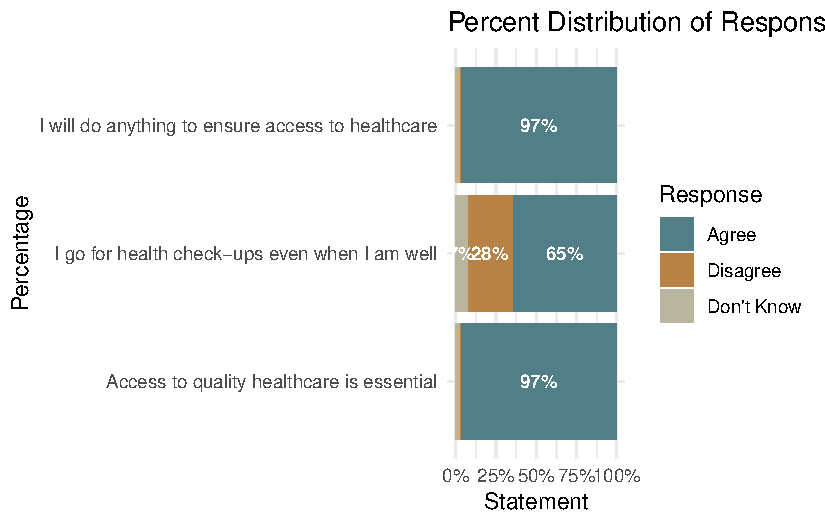
\includegraphics[keepaspectratio]{Utano_report_files/figure-pdf/unnamed-chunk-14-1.pdf}}

The respondents' overwhelming agreement with ``access to quality health
is essential'' and ``I will do anything to ensure access to healthcare''
shows the high value on access to quality healthcare. Such strong
sentiments suggest that the targetted population placess strong
importance on healthcare that is of quality, and is also accessible and
will be willing to engage with service that offers such qualities. ``I
go for health check-ups even when I am well'', which assesses
health-seeking and preventative health behavior, received 65 \%
agreement, 28 \% disagreement, and 7 \% uncertainty, reflecting a more
mixed view compared to the consistently high agreement observed in the
other two statements. This disparity may point to limitations in
preventative health practices, potentially driven by affordability or
access barriers. It suggests that a significant portion of the
population may only seek healthcare when they are already ill, rather
than engaging in routine preventive care.

\pandocbounded{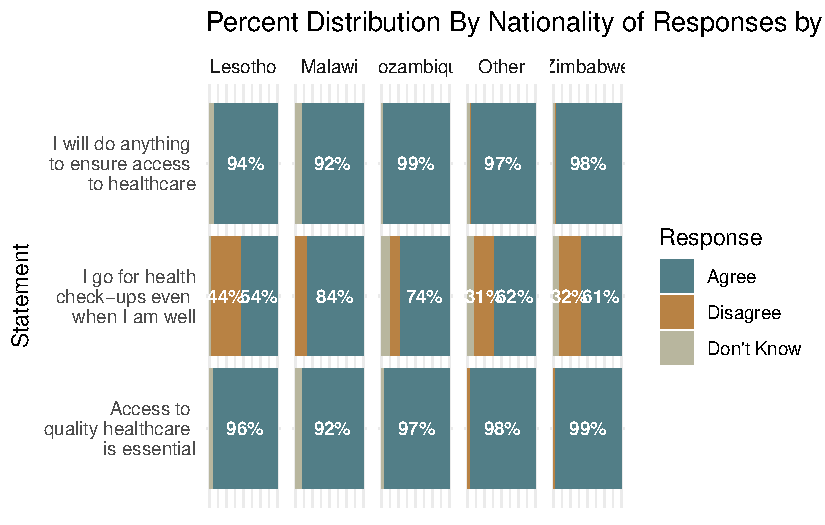
\includegraphics[keepaspectratio]{Utano_report_files/figure-pdf/unnamed-chunk-15-1.pdf}}

An analysis of responses to the healthcare statements by nationality
reflects a consistent emphasis across most groups on the importance of
accessing quality healthcare and ensuring healthcare access. As
presented in Table @@@, Basotho, Zimbabwean, and `Other' nationalities
are notably less likely to seek routine health check-ups compared to
their Malawian and Mozambican counterparts.

\section{SECTION C: Willingness to sign up for the
product.}\label{section-c-willingness-to-sign-up-for-the-product.}

\subsection{Language Preference and Choice of Healthcare
Provider}\label{language-preference-and-choice-of-healthcare-provider}

When asked whether language influences their decision when choosing a
healthcare provider, the majority of respondents affirmed its
importance. Specifically, 88\% of females and 89\% of males agreed that
language plays a role in their decision-making, resulting in an overall
agreement of 88\%. This suggests that language is a key consideration
for both females and males when selecting a healthcare provider,
emphasizing the critical importance of language-concordant care in
health service delivery (Table below)

\global\setlength{\Oldarrayrulewidth}{\arrayrulewidth}

\global\setlength{\Oldtabcolsep}{\tabcolsep}

\setlength{\tabcolsep}{2pt}

\renewcommand*{\arraystretch}{1.5}



\providecommand{\ascline}[3]{\noalign{\global\arrayrulewidth #1}\arrayrulecolor[HTML]{#2}\cline{#3}}

\begin{longtable*}[c]{|p{1.01in}|p{1.08in}|p{1.08in}|p{1.08in}}



\ascline{1.5pt}{666666}{1-4}

\multicolumn{1}{>{\raggedright}m{\dimexpr 1.01in+0\tabcolsep}}{\textcolor[HTML]{000000}{\fontsize{11}{11}\selectfont{\global\setmainfont{Arial}{Language}}}} & \multicolumn{1}{>{\raggedright}m{\dimexpr 1.08in+0\tabcolsep}}{\textcolor[HTML]{000000}{\fontsize{11}{11}\selectfont{\global\setmainfont{Arial}{Female}}}} & \multicolumn{1}{>{\raggedright}m{\dimexpr 1.08in+0\tabcolsep}}{\textcolor[HTML]{000000}{\fontsize{11}{11}\selectfont{\global\setmainfont{Arial}{Male}}}} & \multicolumn{1}{>{\raggedright}m{\dimexpr 1.08in+0\tabcolsep}}{\textcolor[HTML]{000000}{\fontsize{11}{11}\selectfont{\global\setmainfont{Arial}{Total}}}} \\

\ascline{1.5pt}{666666}{1-4}\endfirsthead 

\ascline{1.5pt}{666666}{1-4}

\multicolumn{1}{>{\raggedright}m{\dimexpr 1.01in+0\tabcolsep}}{\textcolor[HTML]{000000}{\fontsize{11}{11}\selectfont{\global\setmainfont{Arial}{Language}}}} & \multicolumn{1}{>{\raggedright}m{\dimexpr 1.08in+0\tabcolsep}}{\textcolor[HTML]{000000}{\fontsize{11}{11}\selectfont{\global\setmainfont{Arial}{Female}}}} & \multicolumn{1}{>{\raggedright}m{\dimexpr 1.08in+0\tabcolsep}}{\textcolor[HTML]{000000}{\fontsize{11}{11}\selectfont{\global\setmainfont{Arial}{Male}}}} & \multicolumn{1}{>{\raggedright}m{\dimexpr 1.08in+0\tabcolsep}}{\textcolor[HTML]{000000}{\fontsize{11}{11}\selectfont{\global\setmainfont{Arial}{Total}}}} \\

\ascline{1.5pt}{666666}{1-4}\endhead



\multicolumn{1}{>{\raggedright}m{\dimexpr 1.01in+0\tabcolsep}}{\textcolor[HTML]{000000}{\fontsize{11}{11}\selectfont{\global\setmainfont{Arial}{Agree}}}} & \multicolumn{1}{>{\raggedright}m{\dimexpr 1.08in+0\tabcolsep}}{\textcolor[HTML]{000000}{\fontsize{11}{11}\selectfont{\global\setmainfont{Arial}{163\ \ (88\%)}}}} & \multicolumn{1}{>{\raggedright}m{\dimexpr 1.08in+0\tabcolsep}}{\textcolor[HTML]{000000}{\fontsize{11}{11}\selectfont{\global\setmainfont{Arial}{160\ \ (89\%)}}}} & \multicolumn{1}{>{\raggedright}m{\dimexpr 1.08in+0\tabcolsep}}{\textcolor[HTML]{000000}{\fontsize{11}{11}\selectfont{\global\setmainfont{Arial}{323\ \ (88\%)}}}} \\





\multicolumn{1}{>{\raggedright}m{\dimexpr 1.01in+0\tabcolsep}}{\textcolor[HTML]{000000}{\fontsize{11}{11}\selectfont{\global\setmainfont{Arial}{Disagree}}}} & \multicolumn{1}{>{\raggedright}m{\dimexpr 1.08in+0\tabcolsep}}{\textcolor[HTML]{000000}{\fontsize{11}{11}\selectfont{\global\setmainfont{Arial}{17\ \ \ (9\%)}}}} & \multicolumn{1}{>{\raggedright}m{\dimexpr 1.08in+0\tabcolsep}}{\textcolor[HTML]{000000}{\fontsize{11}{11}\selectfont{\global\setmainfont{Arial}{13\ \ \ (7\%)}}}} & \multicolumn{1}{>{\raggedright}m{\dimexpr 1.08in+0\tabcolsep}}{\textcolor[HTML]{000000}{\fontsize{11}{11}\selectfont{\global\setmainfont{Arial}{30\ \ \ (8\%)}}}} \\





\multicolumn{1}{>{\raggedright}m{\dimexpr 1.01in+0\tabcolsep}}{\textcolor[HTML]{000000}{\fontsize{11}{11}\selectfont{\global\setmainfont{Arial}{Dont\ know}}}} & \multicolumn{1}{>{\raggedright}m{\dimexpr 1.08in+0\tabcolsep}}{\textcolor[HTML]{000000}{\fontsize{11}{11}\selectfont{\global\setmainfont{Arial}{6\ \ \ (3\%)}}}} & \multicolumn{1}{>{\raggedright}m{\dimexpr 1.08in+0\tabcolsep}}{\textcolor[HTML]{000000}{\fontsize{11}{11}\selectfont{\global\setmainfont{Arial}{7\ \ \ (4\%)}}}} & \multicolumn{1}{>{\raggedright}m{\dimexpr 1.08in+0\tabcolsep}}{\textcolor[HTML]{000000}{\fontsize{11}{11}\selectfont{\global\setmainfont{Arial}{13\ \ \ (4\%)}}}} \\





\multicolumn{1}{>{\raggedright}m{\dimexpr 1.01in+0\tabcolsep}}{\textcolor[HTML]{000000}{\fontsize{11}{11}\selectfont{\global\setmainfont{Arial}{Total}}}} & \multicolumn{1}{>{\raggedright}m{\dimexpr 1.08in+0\tabcolsep}}{\textcolor[HTML]{000000}{\fontsize{11}{11}\selectfont{\global\setmainfont{Arial}{186\ (100\%)}}}} & \multicolumn{1}{>{\raggedright}m{\dimexpr 1.08in+0\tabcolsep}}{\textcolor[HTML]{000000}{\fontsize{11}{11}\selectfont{\global\setmainfont{Arial}{180\ (100\%)}}}} & \multicolumn{1}{>{\raggedright}m{\dimexpr 1.08in+0\tabcolsep}}{\textcolor[HTML]{000000}{\fontsize{11}{11}\selectfont{\global\setmainfont{Arial}{366\ (100\%)}}}} \\

\ascline{1.5pt}{666666}{1-4}



\end{longtable*}



\arrayrulecolor[HTML]{000000}

\global\setlength{\arrayrulewidth}{\Oldarrayrulewidth}

\global\setlength{\tabcolsep}{\Oldtabcolsep}

\renewcommand*{\arraystretch}{1}

\subsection{Gender Preference and Choice of Healthcare
Provider}\label{gender-preference-and-choice-of-healthcare-provider}

When asked whether they choose a healthcare provider based on gender,
61\% of females and 64\% of males agreed with the statement, suggesting
that gender plays a role in provider selection for a significant portion
of both groups. Overall, 62\% of respondents agreed.

\global\setlength{\Oldarrayrulewidth}{\arrayrulewidth}

\global\setlength{\Oldtabcolsep}{\tabcolsep}

\setlength{\tabcolsep}{2pt}

\renewcommand*{\arraystretch}{1.5}



\providecommand{\ascline}[3]{\noalign{\global\arrayrulewidth #1}\arrayrulecolor[HTML]{#2}\cline{#3}}

\begin{longtable*}[c]{|p{1.01in}|p{1.08in}|p{1.08in}|p{1.08in}}



\ascline{1.5pt}{666666}{1-4}

\multicolumn{1}{>{\raggedright}m{\dimexpr 1.01in+0\tabcolsep}}{\textcolor[HTML]{000000}{\fontsize{11}{11}\selectfont{\global\setmainfont{Arial}{Gender}}}} & \multicolumn{1}{>{\raggedright}m{\dimexpr 1.08in+0\tabcolsep}}{\textcolor[HTML]{000000}{\fontsize{11}{11}\selectfont{\global\setmainfont{Arial}{Female}}}} & \multicolumn{1}{>{\raggedright}m{\dimexpr 1.08in+0\tabcolsep}}{\textcolor[HTML]{000000}{\fontsize{11}{11}\selectfont{\global\setmainfont{Arial}{Male}}}} & \multicolumn{1}{>{\raggedright}m{\dimexpr 1.08in+0\tabcolsep}}{\textcolor[HTML]{000000}{\fontsize{11}{11}\selectfont{\global\setmainfont{Arial}{Total}}}} \\

\ascline{1.5pt}{666666}{1-4}\endfirsthead 

\ascline{1.5pt}{666666}{1-4}

\multicolumn{1}{>{\raggedright}m{\dimexpr 1.01in+0\tabcolsep}}{\textcolor[HTML]{000000}{\fontsize{11}{11}\selectfont{\global\setmainfont{Arial}{Gender}}}} & \multicolumn{1}{>{\raggedright}m{\dimexpr 1.08in+0\tabcolsep}}{\textcolor[HTML]{000000}{\fontsize{11}{11}\selectfont{\global\setmainfont{Arial}{Female}}}} & \multicolumn{1}{>{\raggedright}m{\dimexpr 1.08in+0\tabcolsep}}{\textcolor[HTML]{000000}{\fontsize{11}{11}\selectfont{\global\setmainfont{Arial}{Male}}}} & \multicolumn{1}{>{\raggedright}m{\dimexpr 1.08in+0\tabcolsep}}{\textcolor[HTML]{000000}{\fontsize{11}{11}\selectfont{\global\setmainfont{Arial}{Total}}}} \\

\ascline{1.5pt}{666666}{1-4}\endhead



\multicolumn{1}{>{\raggedright}m{\dimexpr 1.01in+0\tabcolsep}}{\textcolor[HTML]{000000}{\fontsize{11}{11}\selectfont{\global\setmainfont{Arial}{Agree}}}} & \multicolumn{1}{>{\raggedright}m{\dimexpr 1.08in+0\tabcolsep}}{\textcolor[HTML]{000000}{\fontsize{11}{11}\selectfont{\global\setmainfont{Arial}{114\ \ (61\%)}}}} & \multicolumn{1}{>{\raggedright}m{\dimexpr 1.08in+0\tabcolsep}}{\textcolor[HTML]{000000}{\fontsize{11}{11}\selectfont{\global\setmainfont{Arial}{114\ \ (64\%)}}}} & \multicolumn{1}{>{\raggedright}m{\dimexpr 1.08in+0\tabcolsep}}{\textcolor[HTML]{000000}{\fontsize{11}{11}\selectfont{\global\setmainfont{Arial}{228\ \ (62\%)}}}} \\





\multicolumn{1}{>{\raggedright}m{\dimexpr 1.01in+0\tabcolsep}}{\textcolor[HTML]{000000}{\fontsize{11}{11}\selectfont{\global\setmainfont{Arial}{Disagree}}}} & \multicolumn{1}{>{\raggedright}m{\dimexpr 1.08in+0\tabcolsep}}{\textcolor[HTML]{000000}{\fontsize{11}{11}\selectfont{\global\setmainfont{Arial}{68\ \ (36\%)}}}} & \multicolumn{1}{>{\raggedright}m{\dimexpr 1.08in+0\tabcolsep}}{\textcolor[HTML]{000000}{\fontsize{11}{11}\selectfont{\global\setmainfont{Arial}{58\ \ (33\%)}}}} & \multicolumn{1}{>{\raggedright}m{\dimexpr 1.08in+0\tabcolsep}}{\textcolor[HTML]{000000}{\fontsize{11}{11}\selectfont{\global\setmainfont{Arial}{126\ \ (35\%)}}}} \\





\multicolumn{1}{>{\raggedright}m{\dimexpr 1.01in+0\tabcolsep}}{\textcolor[HTML]{000000}{\fontsize{11}{11}\selectfont{\global\setmainfont{Arial}{Dont\ know}}}} & \multicolumn{1}{>{\raggedright}m{\dimexpr 1.08in+0\tabcolsep}}{\textcolor[HTML]{000000}{\fontsize{11}{11}\selectfont{\global\setmainfont{Arial}{6\ \ \ (3\%)}}}} & \multicolumn{1}{>{\raggedright}m{\dimexpr 1.08in+0\tabcolsep}}{\textcolor[HTML]{000000}{\fontsize{11}{11}\selectfont{\global\setmainfont{Arial}{5\ \ \ (3\%)}}}} & \multicolumn{1}{>{\raggedright}m{\dimexpr 1.08in+0\tabcolsep}}{\textcolor[HTML]{000000}{\fontsize{11}{11}\selectfont{\global\setmainfont{Arial}{11\ \ \ (3\%)}}}} \\





\multicolumn{1}{>{\raggedright}m{\dimexpr 1.01in+0\tabcolsep}}{\textcolor[HTML]{000000}{\fontsize{11}{11}\selectfont{\global\setmainfont{Arial}{Total}}}} & \multicolumn{1}{>{\raggedright}m{\dimexpr 1.08in+0\tabcolsep}}{\textcolor[HTML]{000000}{\fontsize{11}{11}\selectfont{\global\setmainfont{Arial}{188\ (100\%)}}}} & \multicolumn{1}{>{\raggedright}m{\dimexpr 1.08in+0\tabcolsep}}{\textcolor[HTML]{000000}{\fontsize{11}{11}\selectfont{\global\setmainfont{Arial}{177\ (100\%)}}}} & \multicolumn{1}{>{\raggedright}m{\dimexpr 1.08in+0\tabcolsep}}{\textcolor[HTML]{000000}{\fontsize{11}{11}\selectfont{\global\setmainfont{Arial}{365\ (100\%)}}}} \\

\ascline{1.5pt}{666666}{1-4}



\end{longtable*}



\arrayrulecolor[HTML]{000000}

\global\setlength{\arrayrulewidth}{\Oldarrayrulewidth}

\global\setlength{\tabcolsep}{\Oldtabcolsep}

\renewcommand*{\arraystretch}{1}

\subsection{Choosing a healthcare provider based on Availablity of Key
population
Services}\label{choosing-a-healthcare-provider-based-on-availablity-of-key-population-services}

When considering the availability of key population services as a factor
in choosing a healthcare provider, a majority of respondents across both
genders agreed that it influences their choice. Specifically, 67\% of
females and 78\% of males agreed, resulting in an overall agreement of
73\%. This indicates a strong preference for providers that offer
services tailored to key populations.

\global\setlength{\Oldarrayrulewidth}{\arrayrulewidth}

\global\setlength{\Oldtabcolsep}{\tabcolsep}

\setlength{\tabcolsep}{2pt}

\renewcommand*{\arraystretch}{1.5}



\providecommand{\ascline}[3]{\noalign{\global\arrayrulewidth #1}\arrayrulecolor[HTML]{#2}\cline{#3}}

\begin{longtable*}[c]{|p{1.30in}|p{1.08in}|p{1.08in}|p{1.08in}}



\ascline{1.5pt}{666666}{1-4}

\multicolumn{1}{>{\raggedright}m{\dimexpr 1.3in+0\tabcolsep}}{\textcolor[HTML]{000000}{\fontsize{11}{11}\selectfont{\global\setmainfont{Arial}{Key\ population}}}} & \multicolumn{1}{>{\raggedright}m{\dimexpr 1.08in+0\tabcolsep}}{\textcolor[HTML]{000000}{\fontsize{11}{11}\selectfont{\global\setmainfont{Arial}{Female}}}} & \multicolumn{1}{>{\raggedright}m{\dimexpr 1.08in+0\tabcolsep}}{\textcolor[HTML]{000000}{\fontsize{11}{11}\selectfont{\global\setmainfont{Arial}{Male}}}} & \multicolumn{1}{>{\raggedright}m{\dimexpr 1.08in+0\tabcolsep}}{\textcolor[HTML]{000000}{\fontsize{11}{11}\selectfont{\global\setmainfont{Arial}{Total}}}} \\

\ascline{1.5pt}{666666}{1-4}\endfirsthead 

\ascline{1.5pt}{666666}{1-4}

\multicolumn{1}{>{\raggedright}m{\dimexpr 1.3in+0\tabcolsep}}{\textcolor[HTML]{000000}{\fontsize{11}{11}\selectfont{\global\setmainfont{Arial}{Key\ population}}}} & \multicolumn{1}{>{\raggedright}m{\dimexpr 1.08in+0\tabcolsep}}{\textcolor[HTML]{000000}{\fontsize{11}{11}\selectfont{\global\setmainfont{Arial}{Female}}}} & \multicolumn{1}{>{\raggedright}m{\dimexpr 1.08in+0\tabcolsep}}{\textcolor[HTML]{000000}{\fontsize{11}{11}\selectfont{\global\setmainfont{Arial}{Male}}}} & \multicolumn{1}{>{\raggedright}m{\dimexpr 1.08in+0\tabcolsep}}{\textcolor[HTML]{000000}{\fontsize{11}{11}\selectfont{\global\setmainfont{Arial}{Total}}}} \\

\ascline{1.5pt}{666666}{1-4}\endhead



\multicolumn{1}{>{\raggedright}m{\dimexpr 1.3in+0\tabcolsep}}{\textcolor[HTML]{000000}{\fontsize{11}{11}\selectfont{\global\setmainfont{Arial}{Agree}}}} & \multicolumn{1}{>{\raggedright}m{\dimexpr 1.08in+0\tabcolsep}}{\textcolor[HTML]{000000}{\fontsize{11}{11}\selectfont{\global\setmainfont{Arial}{125\ \ (67\%)}}}} & \multicolumn{1}{>{\raggedright}m{\dimexpr 1.08in+0\tabcolsep}}{\textcolor[HTML]{000000}{\fontsize{11}{11}\selectfont{\global\setmainfont{Arial}{140\ \ (78\%)}}}} & \multicolumn{1}{>{\raggedright}m{\dimexpr 1.08in+0\tabcolsep}}{\textcolor[HTML]{000000}{\fontsize{11}{11}\selectfont{\global\setmainfont{Arial}{265\ \ (73\%)}}}} \\





\multicolumn{1}{>{\raggedright}m{\dimexpr 1.3in+0\tabcolsep}}{\textcolor[HTML]{000000}{\fontsize{11}{11}\selectfont{\global\setmainfont{Arial}{Disagree}}}} & \multicolumn{1}{>{\raggedright}m{\dimexpr 1.08in+0\tabcolsep}}{\textcolor[HTML]{000000}{\fontsize{11}{11}\selectfont{\global\setmainfont{Arial}{32\ \ (17\%)}}}} & \multicolumn{1}{>{\raggedright}m{\dimexpr 1.08in+0\tabcolsep}}{\textcolor[HTML]{000000}{\fontsize{11}{11}\selectfont{\global\setmainfont{Arial}{21\ \ (12\%)}}}} & \multicolumn{1}{>{\raggedright}m{\dimexpr 1.08in+0\tabcolsep}}{\textcolor[HTML]{000000}{\fontsize{11}{11}\selectfont{\global\setmainfont{Arial}{53\ \ (15\%)}}}} \\





\multicolumn{1}{>{\raggedright}m{\dimexpr 1.3in+0\tabcolsep}}{\textcolor[HTML]{000000}{\fontsize{11}{11}\selectfont{\global\setmainfont{Arial}{Dont\ know}}}} & \multicolumn{1}{>{\raggedright}m{\dimexpr 1.08in+0\tabcolsep}}{\textcolor[HTML]{000000}{\fontsize{11}{11}\selectfont{\global\setmainfont{Arial}{29\ \ (16\%)}}}} & \multicolumn{1}{>{\raggedright}m{\dimexpr 1.08in+0\tabcolsep}}{\textcolor[HTML]{000000}{\fontsize{11}{11}\selectfont{\global\setmainfont{Arial}{18\ \ (10\%)}}}} & \multicolumn{1}{>{\raggedright}m{\dimexpr 1.08in+0\tabcolsep}}{\textcolor[HTML]{000000}{\fontsize{11}{11}\selectfont{\global\setmainfont{Arial}{47\ \ (13\%)}}}} \\





\multicolumn{1}{>{\raggedright}m{\dimexpr 1.3in+0\tabcolsep}}{\textcolor[HTML]{000000}{\fontsize{11}{11}\selectfont{\global\setmainfont{Arial}{Total}}}} & \multicolumn{1}{>{\raggedright}m{\dimexpr 1.08in+0\tabcolsep}}{\textcolor[HTML]{000000}{\fontsize{11}{11}\selectfont{\global\setmainfont{Arial}{186\ (100\%)}}}} & \multicolumn{1}{>{\raggedright}m{\dimexpr 1.08in+0\tabcolsep}}{\textcolor[HTML]{000000}{\fontsize{11}{11}\selectfont{\global\setmainfont{Arial}{179\ (100\%)}}}} & \multicolumn{1}{>{\raggedright}m{\dimexpr 1.08in+0\tabcolsep}}{\textcolor[HTML]{000000}{\fontsize{11}{11}\selectfont{\global\setmainfont{Arial}{365\ (100\%)}}}} \\

\ascline{1.5pt}{666666}{1-4}



\end{longtable*}



\arrayrulecolor[HTML]{000000}

\global\setlength{\arrayrulewidth}{\Oldarrayrulewidth}

\global\setlength{\tabcolsep}{\Oldtabcolsep}

\renewcommand*{\arraystretch}{1}

\subsection{Years of Clinical Experience and Choice of Healthcare
Provider}\label{years-of-clinical-experience-and-choice-of-healthcare-provider}

The majority of respondents indicated that years of clinical experience
play a significant role in their choice of healthcare provider. 79\% of
females and 85\% of males agreed with this statement, contributing to an
overall agreement rate of 82\%. This reflects a strong and consistent
preference across both genders for experienced healthcare professionals.

\global\setlength{\Oldarrayrulewidth}{\arrayrulewidth}

\global\setlength{\Oldtabcolsep}{\tabcolsep}

\setlength{\tabcolsep}{2pt}

\renewcommand*{\arraystretch}{1.5}



\providecommand{\ascline}[3]{\noalign{\global\arrayrulewidth #1}\arrayrulecolor[HTML]{#2}\cline{#3}}

\begin{longtable*}[c]{|p{1.64in}|p{1.08in}|p{1.08in}|p{1.08in}}



\ascline{1.5pt}{666666}{1-4}

\multicolumn{1}{>{\raggedright}m{\dimexpr 1.64in+0\tabcolsep}}{\textcolor[HTML]{000000}{\fontsize{11}{11}\selectfont{\global\setmainfont{Arial}{Years\ of\ experience}}}} & \multicolumn{1}{>{\raggedright}m{\dimexpr 1.08in+0\tabcolsep}}{\textcolor[HTML]{000000}{\fontsize{11}{11}\selectfont{\global\setmainfont{Arial}{Female}}}} & \multicolumn{1}{>{\raggedright}m{\dimexpr 1.08in+0\tabcolsep}}{\textcolor[HTML]{000000}{\fontsize{11}{11}\selectfont{\global\setmainfont{Arial}{Male}}}} & \multicolumn{1}{>{\raggedright}m{\dimexpr 1.08in+0\tabcolsep}}{\textcolor[HTML]{000000}{\fontsize{11}{11}\selectfont{\global\setmainfont{Arial}{Total}}}} \\

\ascline{1.5pt}{666666}{1-4}\endfirsthead 

\ascline{1.5pt}{666666}{1-4}

\multicolumn{1}{>{\raggedright}m{\dimexpr 1.64in+0\tabcolsep}}{\textcolor[HTML]{000000}{\fontsize{11}{11}\selectfont{\global\setmainfont{Arial}{Years\ of\ experience}}}} & \multicolumn{1}{>{\raggedright}m{\dimexpr 1.08in+0\tabcolsep}}{\textcolor[HTML]{000000}{\fontsize{11}{11}\selectfont{\global\setmainfont{Arial}{Female}}}} & \multicolumn{1}{>{\raggedright}m{\dimexpr 1.08in+0\tabcolsep}}{\textcolor[HTML]{000000}{\fontsize{11}{11}\selectfont{\global\setmainfont{Arial}{Male}}}} & \multicolumn{1}{>{\raggedright}m{\dimexpr 1.08in+0\tabcolsep}}{\textcolor[HTML]{000000}{\fontsize{11}{11}\selectfont{\global\setmainfont{Arial}{Total}}}} \\

\ascline{1.5pt}{666666}{1-4}\endhead



\multicolumn{1}{>{\raggedright}m{\dimexpr 1.64in+0\tabcolsep}}{\textcolor[HTML]{000000}{\fontsize{11}{11}\selectfont{\global\setmainfont{Arial}{Agree}}}} & \multicolumn{1}{>{\raggedright}m{\dimexpr 1.08in+0\tabcolsep}}{\textcolor[HTML]{000000}{\fontsize{11}{11}\selectfont{\global\setmainfont{Arial}{146\ \ (79\%)}}}} & \multicolumn{1}{>{\raggedright}m{\dimexpr 1.08in+0\tabcolsep}}{\textcolor[HTML]{000000}{\fontsize{11}{11}\selectfont{\global\setmainfont{Arial}{153\ \ (85\%)}}}} & \multicolumn{1}{>{\raggedright}m{\dimexpr 1.08in+0\tabcolsep}}{\textcolor[HTML]{000000}{\fontsize{11}{11}\selectfont{\global\setmainfont{Arial}{299\ \ (82\%)}}}} \\





\multicolumn{1}{>{\raggedright}m{\dimexpr 1.64in+0\tabcolsep}}{\textcolor[HTML]{000000}{\fontsize{11}{11}\selectfont{\global\setmainfont{Arial}{Disagree}}}} & \multicolumn{1}{>{\raggedright}m{\dimexpr 1.08in+0\tabcolsep}}{\textcolor[HTML]{000000}{\fontsize{11}{11}\selectfont{\global\setmainfont{Arial}{31\ \ (17\%)}}}} & \multicolumn{1}{>{\raggedright}m{\dimexpr 1.08in+0\tabcolsep}}{\textcolor[HTML]{000000}{\fontsize{11}{11}\selectfont{\global\setmainfont{Arial}{20\ \ (11\%)}}}} & \multicolumn{1}{>{\raggedright}m{\dimexpr 1.08in+0\tabcolsep}}{\textcolor[HTML]{000000}{\fontsize{11}{11}\selectfont{\global\setmainfont{Arial}{51\ \ (14\%)}}}} \\





\multicolumn{1}{>{\raggedright}m{\dimexpr 1.64in+0\tabcolsep}}{\textcolor[HTML]{000000}{\fontsize{11}{11}\selectfont{\global\setmainfont{Arial}{Dont\ know}}}} & \multicolumn{1}{>{\raggedright}m{\dimexpr 1.08in+0\tabcolsep}}{\textcolor[HTML]{000000}{\fontsize{11}{11}\selectfont{\global\setmainfont{Arial}{7\ \ \ (4\%)}}}} & \multicolumn{1}{>{\raggedright}m{\dimexpr 1.08in+0\tabcolsep}}{\textcolor[HTML]{000000}{\fontsize{11}{11}\selectfont{\global\setmainfont{Arial}{6\ \ \ (3\%)}}}} & \multicolumn{1}{>{\raggedright}m{\dimexpr 1.08in+0\tabcolsep}}{\textcolor[HTML]{000000}{\fontsize{11}{11}\selectfont{\global\setmainfont{Arial}{13\ \ \ (4\%)}}}} \\





\multicolumn{1}{>{\raggedright}m{\dimexpr 1.64in+0\tabcolsep}}{\textcolor[HTML]{000000}{\fontsize{11}{11}\selectfont{\global\setmainfont{Arial}{Total}}}} & \multicolumn{1}{>{\raggedright}m{\dimexpr 1.08in+0\tabcolsep}}{\textcolor[HTML]{000000}{\fontsize{11}{11}\selectfont{\global\setmainfont{Arial}{184\ (100\%)}}}} & \multicolumn{1}{>{\raggedright}m{\dimexpr 1.08in+0\tabcolsep}}{\textcolor[HTML]{000000}{\fontsize{11}{11}\selectfont{\global\setmainfont{Arial}{179\ (100\%)}}}} & \multicolumn{1}{>{\raggedright}m{\dimexpr 1.08in+0\tabcolsep}}{\textcolor[HTML]{000000}{\fontsize{11}{11}\selectfont{\global\setmainfont{Arial}{363\ (100\%)}}}} \\

\ascline{1.5pt}{666666}{1-4}



\end{longtable*}



\arrayrulecolor[HTML]{000000}

\global\setlength{\arrayrulewidth}{\Oldarrayrulewidth}

\global\setlength{\tabcolsep}{\Oldtabcolsep}

\renewcommand*{\arraystretch}{1}

\section{Selecting health services
products}\label{selecting-health-services-products}

Understanding how different genders engage with various service types
can provide valuable insights into consumer preferences and
accessibility. This analysis explores the distribution of male and
female preferences across different service types.The chart highlights a
clear gender difference in service preferences. Females predominantly
chose Gold, Platinum, and Silver services, with Gold being the most
favored. In contrast, males showed a stronger preference for Lithium
services, demonstrating a noticeable skew toward this option. This
pattern suggests potential gender-driven trends that could inform
service customization and marketing strategies

\pandocbounded{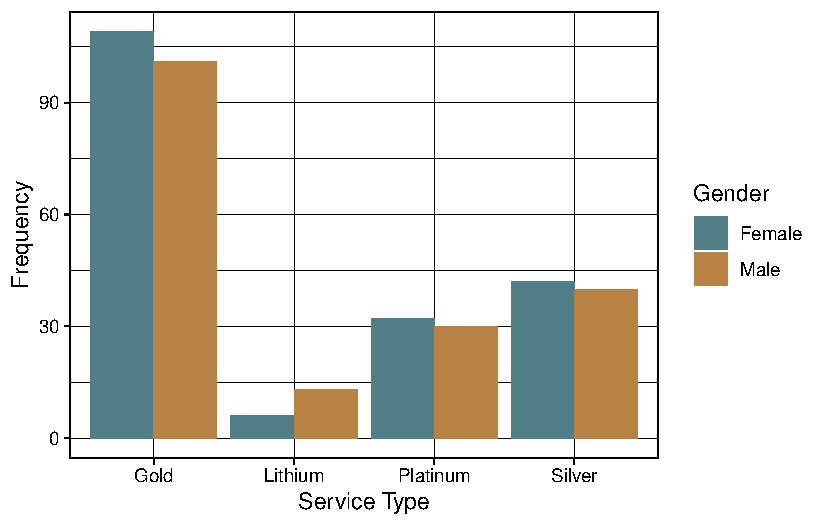
\includegraphics[keepaspectratio]{Utano_report_files/figure-pdf/unnamed-chunk-20-1.pdf}}

Understanding how different Nationality engage with various service
types can provide valuable insights into consumer preferences and
accessibility.The chart below highlights how employment status influence
service preferences. Those in the informal sector predominantly chose
Gold while those in the formal sector,show stronger preference in
Lithium, Platinum and Silver services.

\pandocbounded{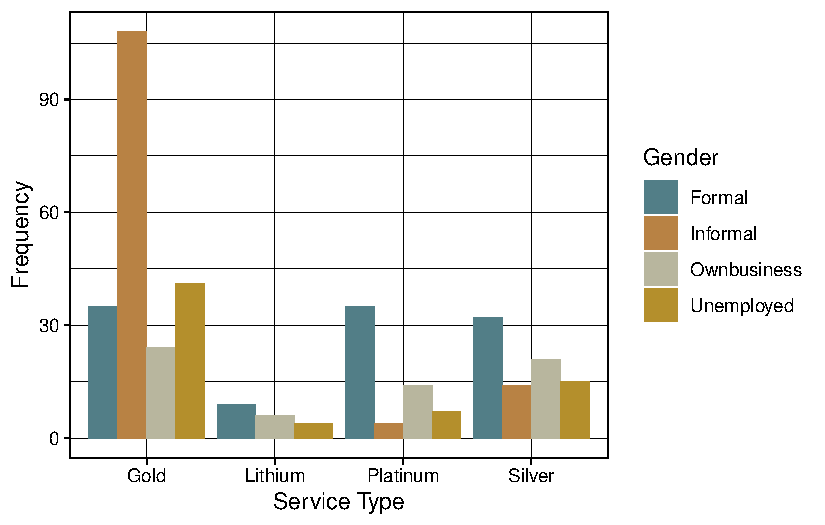
\includegraphics[keepaspectratio]{Utano_report_files/figure-pdf/unnamed-chunk-21-1.pdf}}

\section{Preferred Payment Options}\label{preferred-payment-options}

When asked about their preferred payment method for healthcare services,
cash emerged as the most commonly selected option, with 40\% of
respondents indicating this preference. This was followed by card
payments, selected by 26\%, and insurance, chosen by 21\% of
respondents. Prepaid options were the least preferred, with only 12\% of
participants opting for this method.

\begin{table}
\fontsize{12.0pt}{14.4pt}\selectfont
\begin{tabular*}{\linewidth}{@{\extracolsep{\fill}}lrr}
\toprule
Payment Option & Frequency & Percentage \\ 
\midrule\addlinespace[2.5pt]
Card & 99 & 26\% \\ 
Cash & 152 & 40\% \\ 
Insurance & 81 & 21\% \\ 
Prepaid & 46 & 12\% \\ 
Total & 378 & 100\% \\ 
\bottomrule
\end{tabular*}
\end{table}

When asked about their preferred subscription method for healthcare
services, the majority of respondents (46\%) indicated a preference for
monthly subscriptions, suggesting a favorability toward shorter, more
flexible payment cycles. This was followed by one-time subscriptions at
20\%, and annual subscriptions at 16\%.Less commonly selected were
quarterly and biannual subscriptions, accounting for 12\% and 6\% of
responses, respectively.

\begin{table}
\fontsize{12.0pt}{14.4pt}\selectfont
\begin{tabular*}{\linewidth}{@{\extracolsep{\fill}}lrr}
\toprule
Subscription Option & Frequency & Percentage \\ 
\midrule\addlinespace[2.5pt]
Annual & 60 & 16\% \\ 
Biannual & 22 & 6\% \\ 
Monthly & 172 & 46\% \\ 
Once & 76 & 20\% \\ 
Quarterly & 46 & 12\% \\ 
Total & 376 & 100\% \\ 
\bottomrule
\end{tabular*}
\end{table}

When asked about their preferred method of subscribing to a healthcare
service, 44\% of respondents favored an assisted subscription,
indicating a preference for guided or in-person support. Online
subscriptions were selected by 35\%, demonstrating a growing acceptance
of digital platforms for managing healthcare enrollment. Meanwhile, 21\%
preferred to subscribe through their employer.

\begin{table}
\fontsize{12.0pt}{14.4pt}\selectfont
\begin{tabular*}{\linewidth}{@{\extracolsep{\fill}}lrr}
\toprule
Subscription Method & Frequency & Percentage \\ 
\midrule\addlinespace[2.5pt]
Assisted & 167 & 44\% \\ 
Employer & 80 & 21\% \\ 
Online & 132 & 35\% \\ 
Total & 379 & 100\% \\ 
\bottomrule
\end{tabular*}
\end{table}

\begin{table}
\fontsize{12.0pt}{14.4pt}\selectfont
\begin{tabular*}{\linewidth}{@{\extracolsep{\fill}}lrr}
\toprule
Employer & Frequency & Percentage \\ 
\midrule\addlinespace[2.5pt]
I am not an employer & 184 & 49\% \\ 
No & 24 & 6\% \\ 
Yes & 169 & 45\% \\ 
Total & 377 & 100\% \\ 
\bottomrule
\end{tabular*}
\end{table}

\global\setlength{\Oldarrayrulewidth}{\arrayrulewidth}

\global\setlength{\Oldtabcolsep}{\tabcolsep}

\setlength{\tabcolsep}{2pt}

\renewcommand*{\arraystretch}{1.5}



\providecommand{\ascline}[3]{\noalign{\global\arrayrulewidth #1}\arrayrulecolor[HTML]{#2}\cline{#3}}

\begin{longtable*}[c]{|p{1.72in}|p{0.99in}|p{0.93in}|p{0.99in}|p{1.08in}}



\ascline{1.5pt}{666666}{1-5}

\multicolumn{1}{>{\raggedright}m{\dimexpr 1.72in+0\tabcolsep}}{\textcolor[HTML]{000000}{\fontsize{11}{11}\selectfont{\global\setmainfont{Arial}{Employer}}}} & \multicolumn{1}{>{\raggedright}m{\dimexpr 0.99in+0\tabcolsep}}{\textcolor[HTML]{000000}{\fontsize{11}{11}\selectfont{\global\setmainfont{Arial}{Assisted}}}} & \multicolumn{1}{>{\raggedright}m{\dimexpr 0.93in+0\tabcolsep}}{\textcolor[HTML]{000000}{\fontsize{11}{11}\selectfont{\global\setmainfont{Arial}{Employer}}}} & \multicolumn{1}{>{\raggedright}m{\dimexpr 0.99in+0\tabcolsep}}{\textcolor[HTML]{000000}{\fontsize{11}{11}\selectfont{\global\setmainfont{Arial}{Online}}}} & \multicolumn{1}{>{\raggedright}m{\dimexpr 1.08in+0\tabcolsep}}{\textcolor[HTML]{000000}{\fontsize{11}{11}\selectfont{\global\setmainfont{Arial}{Total}}}} \\

\ascline{1.5pt}{666666}{1-5}\endfirsthead 

\ascline{1.5pt}{666666}{1-5}

\multicolumn{1}{>{\raggedright}m{\dimexpr 1.72in+0\tabcolsep}}{\textcolor[HTML]{000000}{\fontsize{11}{11}\selectfont{\global\setmainfont{Arial}{Employer}}}} & \multicolumn{1}{>{\raggedright}m{\dimexpr 0.99in+0\tabcolsep}}{\textcolor[HTML]{000000}{\fontsize{11}{11}\selectfont{\global\setmainfont{Arial}{Assisted}}}} & \multicolumn{1}{>{\raggedright}m{\dimexpr 0.93in+0\tabcolsep}}{\textcolor[HTML]{000000}{\fontsize{11}{11}\selectfont{\global\setmainfont{Arial}{Employer}}}} & \multicolumn{1}{>{\raggedright}m{\dimexpr 0.99in+0\tabcolsep}}{\textcolor[HTML]{000000}{\fontsize{11}{11}\selectfont{\global\setmainfont{Arial}{Online}}}} & \multicolumn{1}{>{\raggedright}m{\dimexpr 1.08in+0\tabcolsep}}{\textcolor[HTML]{000000}{\fontsize{11}{11}\selectfont{\global\setmainfont{Arial}{Total}}}} \\

\ascline{1.5pt}{666666}{1-5}\endhead



\multicolumn{1}{>{\raggedright}m{\dimexpr 1.72in+0\tabcolsep}}{\textcolor[HTML]{000000}{\fontsize{11}{11}\selectfont{\global\setmainfont{Arial}{I\ am\ not\ an\ employer}}}} & \multicolumn{1}{>{\raggedright}m{\dimexpr 0.99in+0\tabcolsep}}{\textcolor[HTML]{000000}{\fontsize{11}{11}\selectfont{\global\setmainfont{Arial}{73\ (40\%)}}}} & \multicolumn{1}{>{\raggedright}m{\dimexpr 0.93in+0\tabcolsep}}{\textcolor[HTML]{000000}{\fontsize{11}{11}\selectfont{\global\setmainfont{Arial}{48\ (26\%)}}}} & \multicolumn{1}{>{\raggedright}m{\dimexpr 0.99in+0\tabcolsep}}{\textcolor[HTML]{000000}{\fontsize{11}{11}\selectfont{\global\setmainfont{Arial}{62\ (34\%)}}}} & \multicolumn{1}{>{\raggedright}m{\dimexpr 1.08in+0\tabcolsep}}{\textcolor[HTML]{000000}{\fontsize{11}{11}\selectfont{\global\setmainfont{Arial}{183\ (100\%)}}}} \\





\multicolumn{1}{>{\raggedright}m{\dimexpr 1.72in+0\tabcolsep}}{\textcolor[HTML]{000000}{\fontsize{11}{11}\selectfont{\global\setmainfont{Arial}{No}}}} & \multicolumn{1}{>{\raggedright}m{\dimexpr 0.99in+0\tabcolsep}}{\textcolor[HTML]{000000}{\fontsize{11}{11}\selectfont{\global\setmainfont{Arial}{14\ (58\%)}}}} & \multicolumn{1}{>{\raggedright}m{\dimexpr 0.93in+0\tabcolsep}}{\textcolor[HTML]{000000}{\fontsize{11}{11}\selectfont{\global\setmainfont{Arial}{4\ (17\%)}}}} & \multicolumn{1}{>{\raggedright}m{\dimexpr 0.99in+0\tabcolsep}}{\textcolor[HTML]{000000}{\fontsize{11}{11}\selectfont{\global\setmainfont{Arial}{6\ (25\%)}}}} & \multicolumn{1}{>{\raggedright}m{\dimexpr 1.08in+0\tabcolsep}}{\textcolor[HTML]{000000}{\fontsize{11}{11}\selectfont{\global\setmainfont{Arial}{24\ (100\%)}}}} \\





\multicolumn{1}{>{\raggedright}m{\dimexpr 1.72in+0\tabcolsep}}{\textcolor[HTML]{000000}{\fontsize{11}{11}\selectfont{\global\setmainfont{Arial}{Yes}}}} & \multicolumn{1}{>{\raggedright}m{\dimexpr 0.99in+0\tabcolsep}}{\textcolor[HTML]{000000}{\fontsize{11}{11}\selectfont{\global\setmainfont{Arial}{77\ (46\%)}}}} & \multicolumn{1}{>{\raggedright}m{\dimexpr 0.93in+0\tabcolsep}}{\textcolor[HTML]{000000}{\fontsize{11}{11}\selectfont{\global\setmainfont{Arial}{27\ (16\%)}}}} & \multicolumn{1}{>{\raggedright}m{\dimexpr 0.99in+0\tabcolsep}}{\textcolor[HTML]{000000}{\fontsize{11}{11}\selectfont{\global\setmainfont{Arial}{62\ (37\%)}}}} & \multicolumn{1}{>{\raggedright}m{\dimexpr 1.08in+0\tabcolsep}}{\textcolor[HTML]{000000}{\fontsize{11}{11}\selectfont{\global\setmainfont{Arial}{166\ (100\%)}}}} \\





\multicolumn{1}{>{\raggedright}m{\dimexpr 1.72in+0\tabcolsep}}{\textcolor[HTML]{000000}{\fontsize{11}{11}\selectfont{\global\setmainfont{Arial}{Total}}}} & \multicolumn{1}{>{\raggedright}m{\dimexpr 0.99in+0\tabcolsep}}{\textcolor[HTML]{000000}{\fontsize{11}{11}\selectfont{\global\setmainfont{Arial}{164\ (44\%)}}}} & \multicolumn{1}{>{\raggedright}m{\dimexpr 0.93in+0\tabcolsep}}{\textcolor[HTML]{000000}{\fontsize{11}{11}\selectfont{\global\setmainfont{Arial}{79\ (21\%)}}}} & \multicolumn{1}{>{\raggedright}m{\dimexpr 0.99in+0\tabcolsep}}{\textcolor[HTML]{000000}{\fontsize{11}{11}\selectfont{\global\setmainfont{Arial}{130\ (35\%)}}}} & \multicolumn{1}{>{\raggedright}m{\dimexpr 1.08in+0\tabcolsep}}{\textcolor[HTML]{000000}{\fontsize{11}{11}\selectfont{\global\setmainfont{Arial}{373\ (100\%)}}}} \\

\ascline{1.5pt}{666666}{1-5}



\end{longtable*}



\arrayrulecolor[HTML]{000000}

\global\setlength{\arrayrulewidth}{\Oldarrayrulewidth}

\global\setlength{\tabcolsep}{\Oldtabcolsep}

\renewcommand*{\arraystretch}{1}

Among respondents who indicated they are currently employers, a
significant majority---95\% (153 individuals)---reported that they would
be willing to obtain insurance coverage for their employees if offered a
plan that costs less than their current payment. Only 5\% (8
individuals) expressed reluctance to make such a
change.Furthermore,Among 167 employers surveyed, the majority---56\%
(93)---indicated they would choose the Gold package for their employees,
reflecting a strong preference for premium coverage. This was followed
by Silver (24\%), Platinum (16\%), and Lithium (5\%).

\global\setlength{\Oldarrayrulewidth}{\arrayrulewidth}

\global\setlength{\Oldtabcolsep}{\tabcolsep}

\setlength{\tabcolsep}{2pt}

\renewcommand*{\arraystretch}{1.5}



\providecommand{\ascline}[3]{\noalign{\global\arrayrulewidth #1}\arrayrulecolor[HTML]{#2}\cline{#3}}

\begin{longtable*}[c]{|p{0.91in}|p{0.91in}|p{0.88in}|p{0.91in}|p{0.91in}|p{0.91in}|p{1.08in}}



\ascline{1.5pt}{666666}{1-7}

\multicolumn{1}{>{\raggedright}m{\dimexpr 0.91in+0\tabcolsep}}{\textcolor[HTML]{000000}{\fontsize{11}{11}\selectfont{\global\setmainfont{Arial}{Employer}}}} & \multicolumn{1}{>{\raggedright}m{\dimexpr 0.91in+0\tabcolsep}}{\textcolor[HTML]{000000}{\fontsize{11}{11}\selectfont{\global\setmainfont{Arial}{Annual}}}} & \multicolumn{1}{>{\raggedright}m{\dimexpr 0.88in+0\tabcolsep}}{\textcolor[HTML]{000000}{\fontsize{11}{11}\selectfont{\global\setmainfont{Arial}{Biannual}}}} & \multicolumn{1}{>{\raggedright}m{\dimexpr 0.91in+0\tabcolsep}}{\textcolor[HTML]{000000}{\fontsize{11}{11}\selectfont{\global\setmainfont{Arial}{Monthly}}}} & \multicolumn{1}{>{\raggedright}m{\dimexpr 0.91in+0\tabcolsep}}{\textcolor[HTML]{000000}{\fontsize{11}{11}\selectfont{\global\setmainfont{Arial}{Once}}}} & \multicolumn{1}{>{\raggedright}m{\dimexpr 0.91in+0\tabcolsep}}{\textcolor[HTML]{000000}{\fontsize{11}{11}\selectfont{\global\setmainfont{Arial}{Quarterly}}}} & \multicolumn{1}{>{\raggedright}m{\dimexpr 1.08in+0\tabcolsep}}{\textcolor[HTML]{000000}{\fontsize{11}{11}\selectfont{\global\setmainfont{Arial}{Total}}}} \\

\ascline{1.5pt}{666666}{1-7}\endfirsthead 

\ascline{1.5pt}{666666}{1-7}

\multicolumn{1}{>{\raggedright}m{\dimexpr 0.91in+0\tabcolsep}}{\textcolor[HTML]{000000}{\fontsize{11}{11}\selectfont{\global\setmainfont{Arial}{Employer}}}} & \multicolumn{1}{>{\raggedright}m{\dimexpr 0.91in+0\tabcolsep}}{\textcolor[HTML]{000000}{\fontsize{11}{11}\selectfont{\global\setmainfont{Arial}{Annual}}}} & \multicolumn{1}{>{\raggedright}m{\dimexpr 0.88in+0\tabcolsep}}{\textcolor[HTML]{000000}{\fontsize{11}{11}\selectfont{\global\setmainfont{Arial}{Biannual}}}} & \multicolumn{1}{>{\raggedright}m{\dimexpr 0.91in+0\tabcolsep}}{\textcolor[HTML]{000000}{\fontsize{11}{11}\selectfont{\global\setmainfont{Arial}{Monthly}}}} & \multicolumn{1}{>{\raggedright}m{\dimexpr 0.91in+0\tabcolsep}}{\textcolor[HTML]{000000}{\fontsize{11}{11}\selectfont{\global\setmainfont{Arial}{Once}}}} & \multicolumn{1}{>{\raggedright}m{\dimexpr 0.91in+0\tabcolsep}}{\textcolor[HTML]{000000}{\fontsize{11}{11}\selectfont{\global\setmainfont{Arial}{Quarterly}}}} & \multicolumn{1}{>{\raggedright}m{\dimexpr 1.08in+0\tabcolsep}}{\textcolor[HTML]{000000}{\fontsize{11}{11}\selectfont{\global\setmainfont{Arial}{Total}}}} \\

\ascline{1.5pt}{666666}{1-7}\endhead



\multicolumn{1}{>{\raggedright}m{\dimexpr 0.91in+0\tabcolsep}}{\textcolor[HTML]{000000}{\fontsize{11}{11}\selectfont{\global\setmainfont{Arial}{Yes}}}} & \multicolumn{1}{>{\raggedright}m{\dimexpr 0.91in+0\tabcolsep}}{\textcolor[HTML]{000000}{\fontsize{11}{11}\selectfont{\global\setmainfont{Arial}{18\ (11\%)}}}} & \multicolumn{1}{>{\raggedright}m{\dimexpr 0.88in+0\tabcolsep}}{\textcolor[HTML]{000000}{\fontsize{11}{11}\selectfont{\global\setmainfont{Arial}{9\ (5\%)}}}} & \multicolumn{1}{>{\raggedright}m{\dimexpr 0.91in+0\tabcolsep}}{\textcolor[HTML]{000000}{\fontsize{11}{11}\selectfont{\global\setmainfont{Arial}{95\ (57\%)}}}} & \multicolumn{1}{>{\raggedright}m{\dimexpr 0.91in+0\tabcolsep}}{\textcolor[HTML]{000000}{\fontsize{11}{11}\selectfont{\global\setmainfont{Arial}{28\ (17\%)}}}} & \multicolumn{1}{>{\raggedright}m{\dimexpr 0.91in+0\tabcolsep}}{\textcolor[HTML]{000000}{\fontsize{11}{11}\selectfont{\global\setmainfont{Arial}{16\ (10\%)}}}} & \multicolumn{1}{>{\raggedright}m{\dimexpr 1.08in+0\tabcolsep}}{\textcolor[HTML]{000000}{\fontsize{11}{11}\selectfont{\global\setmainfont{Arial}{166\ (100\%)}}}} \\

\ascline{1.5pt}{666666}{1-7}



\end{longtable*}



\arrayrulecolor[HTML]{000000}

\global\setlength{\arrayrulewidth}{\Oldarrayrulewidth}

\global\setlength{\tabcolsep}{\Oldtabcolsep}

\renewcommand*{\arraystretch}{1}

\global\setlength{\Oldarrayrulewidth}{\arrayrulewidth}

\global\setlength{\Oldtabcolsep}{\tabcolsep}

\setlength{\tabcolsep}{2pt}

\renewcommand*{\arraystretch}{1.5}



\providecommand{\ascline}[3]{\noalign{\global\arrayrulewidth #1}\arrayrulecolor[HTML]{#2}\cline{#3}}

\begin{longtable*}[c]{|p{0.91in}|p{0.91in}|p{0.78in}|p{0.91in}|p{0.91in}|p{1.08in}}



\ascline{1.5pt}{666666}{1-6}

\multicolumn{1}{>{\raggedright}m{\dimexpr 0.91in+0\tabcolsep}}{\textcolor[HTML]{000000}{\fontsize{11}{11}\selectfont{\global\setmainfont{Arial}{Employer}}}} & \multicolumn{1}{>{\raggedright}m{\dimexpr 0.91in+0\tabcolsep}}{\textcolor[HTML]{000000}{\fontsize{11}{11}\selectfont{\global\setmainfont{Arial}{Gold}}}} & \multicolumn{1}{>{\raggedright}m{\dimexpr 0.78in+0\tabcolsep}}{\textcolor[HTML]{000000}{\fontsize{11}{11}\selectfont{\global\setmainfont{Arial}{Lithium}}}} & \multicolumn{1}{>{\raggedright}m{\dimexpr 0.91in+0\tabcolsep}}{\textcolor[HTML]{000000}{\fontsize{11}{11}\selectfont{\global\setmainfont{Arial}{Platinum}}}} & \multicolumn{1}{>{\raggedright}m{\dimexpr 0.91in+0\tabcolsep}}{\textcolor[HTML]{000000}{\fontsize{11}{11}\selectfont{\global\setmainfont{Arial}{Silver}}}} & \multicolumn{1}{>{\raggedright}m{\dimexpr 1.08in+0\tabcolsep}}{\textcolor[HTML]{000000}{\fontsize{11}{11}\selectfont{\global\setmainfont{Arial}{Total}}}} \\

\ascline{1.5pt}{666666}{1-6}\endfirsthead 

\ascline{1.5pt}{666666}{1-6}

\multicolumn{1}{>{\raggedright}m{\dimexpr 0.91in+0\tabcolsep}}{\textcolor[HTML]{000000}{\fontsize{11}{11}\selectfont{\global\setmainfont{Arial}{Employer}}}} & \multicolumn{1}{>{\raggedright}m{\dimexpr 0.91in+0\tabcolsep}}{\textcolor[HTML]{000000}{\fontsize{11}{11}\selectfont{\global\setmainfont{Arial}{Gold}}}} & \multicolumn{1}{>{\raggedright}m{\dimexpr 0.78in+0\tabcolsep}}{\textcolor[HTML]{000000}{\fontsize{11}{11}\selectfont{\global\setmainfont{Arial}{Lithium}}}} & \multicolumn{1}{>{\raggedright}m{\dimexpr 0.91in+0\tabcolsep}}{\textcolor[HTML]{000000}{\fontsize{11}{11}\selectfont{\global\setmainfont{Arial}{Platinum}}}} & \multicolumn{1}{>{\raggedright}m{\dimexpr 0.91in+0\tabcolsep}}{\textcolor[HTML]{000000}{\fontsize{11}{11}\selectfont{\global\setmainfont{Arial}{Silver}}}} & \multicolumn{1}{>{\raggedright}m{\dimexpr 1.08in+0\tabcolsep}}{\textcolor[HTML]{000000}{\fontsize{11}{11}\selectfont{\global\setmainfont{Arial}{Total}}}} \\

\ascline{1.5pt}{666666}{1-6}\endhead



\multicolumn{1}{>{\raggedright}m{\dimexpr 0.91in+0\tabcolsep}}{\textcolor[HTML]{000000}{\fontsize{11}{11}\selectfont{\global\setmainfont{Arial}{Yes}}}} & \multicolumn{1}{>{\raggedright}m{\dimexpr 0.91in+0\tabcolsep}}{\textcolor[HTML]{000000}{\fontsize{11}{11}\selectfont{\global\setmainfont{Arial}{93\ (56\%)}}}} & \multicolumn{1}{>{\raggedright}m{\dimexpr 0.78in+0\tabcolsep}}{\textcolor[HTML]{000000}{\fontsize{11}{11}\selectfont{\global\setmainfont{Arial}{8\ (5\%)}}}} & \multicolumn{1}{>{\raggedright}m{\dimexpr 0.91in+0\tabcolsep}}{\textcolor[HTML]{000000}{\fontsize{11}{11}\selectfont{\global\setmainfont{Arial}{26\ (16\%)}}}} & \multicolumn{1}{>{\raggedright}m{\dimexpr 0.91in+0\tabcolsep}}{\textcolor[HTML]{000000}{\fontsize{11}{11}\selectfont{\global\setmainfont{Arial}{40\ (24\%)}}}} & \multicolumn{1}{>{\raggedright}m{\dimexpr 1.08in+0\tabcolsep}}{\textcolor[HTML]{000000}{\fontsize{11}{11}\selectfont{\global\setmainfont{Arial}{167\ (100\%)}}}} \\

\ascline{1.5pt}{666666}{1-6}



\end{longtable*}



\arrayrulecolor[HTML]{000000}

\global\setlength{\arrayrulewidth}{\Oldarrayrulewidth}

\global\setlength{\tabcolsep}{\Oldtabcolsep}

\renewcommand*{\arraystretch}{1}

Among respondents who indicated they are currently employers, a
significant majority---95\% (153 individuals)---reported that they would
be willing to obtain insurance coverage for their employees if offered a
plan that costs less than their current payment. Only 5\% (8
individuals) expressed reluctance to make such a change.

\pandocbounded{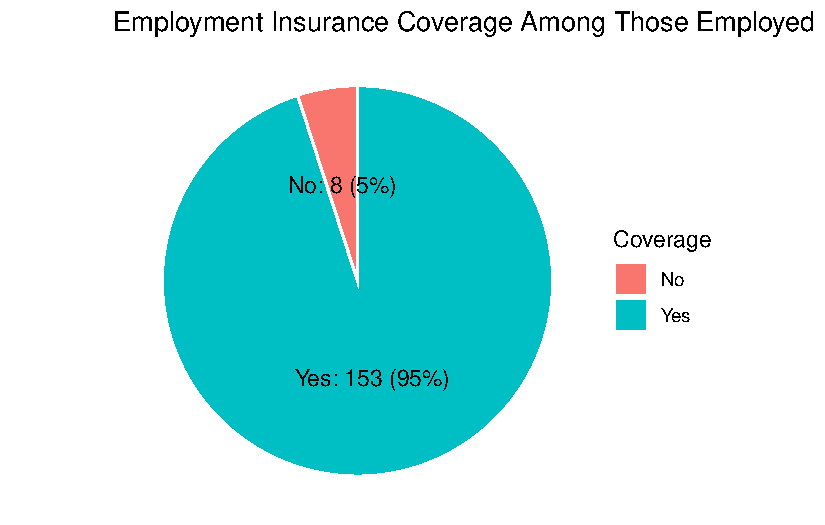
\includegraphics[keepaspectratio]{Utano_report_files/figure-pdf/unnamed-chunk-27-1.pdf}}

A total of 376 subscriptions were recorded. Most were in the 100+ ZAR
(129; 34\%) and 50--59 ZAR (75; 20\%) ranges, followed by 10--19 ZAR
(65; 17\%), 30--39 ZAR (45; 12\%), 20--29 ZAR (41; 11\%), and 40--49 ZAR
(21; 6\%). Within the 100+ ZAR range, online accounted for 57 (44\%),
assisted 49 (30\%), and employer 23 (29\%). In the 50--59 ZAR band,
assisted made up 34 (21\%), employer 17 (21\%), and online 24 (18\%).
Lower price tiers were dominated by assisted subscriptions, especially
in the 10--19 ZAR category with 38 (23\%). Online subscriptions
increased progressively with price, peaking in the highest bracket.

\global\setlength{\Oldarrayrulewidth}{\arrayrulewidth}

\global\setlength{\Oldtabcolsep}{\tabcolsep}

\setlength{\tabcolsep}{2pt}

\renewcommand*{\arraystretch}{1.5}



\providecommand{\ascline}[3]{\noalign{\global\arrayrulewidth #1}\arrayrulecolor[HTML]{#2}\cline{#3}}

\begin{longtable*}[c]{|p{1.68in}|p{1.08in}|p{1.08in}|p{1.08in}|p{1.08in}|p{1.08in}|p{1.24in}}



\ascline{1.5pt}{666666}{1-7}

\multicolumn{1}{>{\raggedright}m{\dimexpr 1.68in+0\tabcolsep}}{\textcolor[HTML]{000000}{\fontsize{11}{11}\selectfont{\global\setmainfont{Arial}{Subscription\ Method}}}} & \multicolumn{1}{>{\raggedright}m{\dimexpr 1.08in+0\tabcolsep}}{\textcolor[HTML]{000000}{\fontsize{11}{11}\selectfont{\global\setmainfont{Arial}{10-19\ ZAR}}}} & \multicolumn{1}{>{\raggedright}m{\dimexpr 1.08in+0\tabcolsep}}{\textcolor[HTML]{000000}{\fontsize{11}{11}\selectfont{\global\setmainfont{Arial}{20-29\ ZAR}}}} & \multicolumn{1}{>{\raggedright}m{\dimexpr 1.08in+0\tabcolsep}}{\textcolor[HTML]{000000}{\fontsize{11}{11}\selectfont{\global\setmainfont{Arial}{30-39\ ZAR}}}} & \multicolumn{1}{>{\raggedright}m{\dimexpr 1.08in+0\tabcolsep}}{\textcolor[HTML]{000000}{\fontsize{11}{11}\selectfont{\global\setmainfont{Arial}{40-49\ ZAR}}}} & \multicolumn{1}{>{\raggedright}m{\dimexpr 1.08in+0\tabcolsep}}{\textcolor[HTML]{000000}{\fontsize{11}{11}\selectfont{\global\setmainfont{Arial}{50-59\ ZAR}}}} & \multicolumn{1}{>{\raggedright}m{\dimexpr 1.24in+0\tabcolsep}}{\textcolor[HTML]{000000}{\fontsize{11}{11}\selectfont{\global\setmainfont{Arial}{100+\ ZAR}}}} \\

\ascline{1.5pt}{666666}{1-7}\endfirsthead 

\ascline{1.5pt}{666666}{1-7}

\multicolumn{1}{>{\raggedright}m{\dimexpr 1.68in+0\tabcolsep}}{\textcolor[HTML]{000000}{\fontsize{11}{11}\selectfont{\global\setmainfont{Arial}{Subscription\ Method}}}} & \multicolumn{1}{>{\raggedright}m{\dimexpr 1.08in+0\tabcolsep}}{\textcolor[HTML]{000000}{\fontsize{11}{11}\selectfont{\global\setmainfont{Arial}{10-19\ ZAR}}}} & \multicolumn{1}{>{\raggedright}m{\dimexpr 1.08in+0\tabcolsep}}{\textcolor[HTML]{000000}{\fontsize{11}{11}\selectfont{\global\setmainfont{Arial}{20-29\ ZAR}}}} & \multicolumn{1}{>{\raggedright}m{\dimexpr 1.08in+0\tabcolsep}}{\textcolor[HTML]{000000}{\fontsize{11}{11}\selectfont{\global\setmainfont{Arial}{30-39\ ZAR}}}} & \multicolumn{1}{>{\raggedright}m{\dimexpr 1.08in+0\tabcolsep}}{\textcolor[HTML]{000000}{\fontsize{11}{11}\selectfont{\global\setmainfont{Arial}{40-49\ ZAR}}}} & \multicolumn{1}{>{\raggedright}m{\dimexpr 1.08in+0\tabcolsep}}{\textcolor[HTML]{000000}{\fontsize{11}{11}\selectfont{\global\setmainfont{Arial}{50-59\ ZAR}}}} & \multicolumn{1}{>{\raggedright}m{\dimexpr 1.24in+0\tabcolsep}}{\textcolor[HTML]{000000}{\fontsize{11}{11}\selectfont{\global\setmainfont{Arial}{100+\ ZAR}}}} \\

\ascline{1.5pt}{666666}{1-7}\endhead



\multicolumn{1}{>{\raggedright}m{\dimexpr 1.68in+0\tabcolsep}}{\textcolor[HTML]{000000}{\fontsize{11}{11}\selectfont{\global\setmainfont{Arial}{Assisted}}}} & \multicolumn{1}{>{\raggedright}m{\dimexpr 1.08in+0\tabcolsep}}{\textcolor[HTML]{000000}{\fontsize{11}{11}\selectfont{\global\setmainfont{Arial}{38\ (3800\%)}}}} & \multicolumn{1}{>{\raggedright}m{\dimexpr 1.08in+0\tabcolsep}}{\textcolor[HTML]{000000}{\fontsize{11}{11}\selectfont{\global\setmainfont{Arial}{18\ (1800\%)}}}} & \multicolumn{1}{>{\raggedright}m{\dimexpr 1.08in+0\tabcolsep}}{\textcolor[HTML]{000000}{\fontsize{11}{11}\selectfont{\global\setmainfont{Arial}{18\ (1800\%)}}}} & \multicolumn{1}{>{\raggedright}m{\dimexpr 1.08in+0\tabcolsep}}{\textcolor[HTML]{000000}{\fontsize{11}{11}\selectfont{\global\setmainfont{Arial}{8\ \ (800\%)}}}} & \multicolumn{1}{>{\raggedright}m{\dimexpr 1.08in+0\tabcolsep}}{\textcolor[HTML]{000000}{\fontsize{11}{11}\selectfont{\global\setmainfont{Arial}{34\ (3400\%)}}}} & \multicolumn{1}{>{\raggedright}m{\dimexpr 1.24in+0\tabcolsep}}{\textcolor[HTML]{000000}{\fontsize{11}{11}\selectfont{\global\setmainfont{Arial}{49\ \ (4900\%)}}}} \\





\multicolumn{1}{>{\raggedright}m{\dimexpr 1.68in+0\tabcolsep}}{\textcolor[HTML]{000000}{\fontsize{11}{11}\selectfont{\global\setmainfont{Arial}{Employer}}}} & \multicolumn{1}{>{\raggedright}m{\dimexpr 1.08in+0\tabcolsep}}{\textcolor[HTML]{000000}{\fontsize{11}{11}\selectfont{\global\setmainfont{Arial}{17\ (1700\%)}}}} & \multicolumn{1}{>{\raggedright}m{\dimexpr 1.08in+0\tabcolsep}}{\textcolor[HTML]{000000}{\fontsize{11}{11}\selectfont{\global\setmainfont{Arial}{11\ (1100\%)}}}} & \multicolumn{1}{>{\raggedright}m{\dimexpr 1.08in+0\tabcolsep}}{\textcolor[HTML]{000000}{\fontsize{11}{11}\selectfont{\global\setmainfont{Arial}{10\ (1000\%)}}}} & \multicolumn{1}{>{\raggedright}m{\dimexpr 1.08in+0\tabcolsep}}{\textcolor[HTML]{000000}{\fontsize{11}{11}\selectfont{\global\setmainfont{Arial}{2\ \ (200\%)}}}} & \multicolumn{1}{>{\raggedright}m{\dimexpr 1.08in+0\tabcolsep}}{\textcolor[HTML]{000000}{\fontsize{11}{11}\selectfont{\global\setmainfont{Arial}{17\ (1700\%)}}}} & \multicolumn{1}{>{\raggedright}m{\dimexpr 1.24in+0\tabcolsep}}{\textcolor[HTML]{000000}{\fontsize{11}{11}\selectfont{\global\setmainfont{Arial}{23\ \ (2300\%)}}}} \\





\multicolumn{1}{>{\raggedright}m{\dimexpr 1.68in+0\tabcolsep}}{\textcolor[HTML]{000000}{\fontsize{11}{11}\selectfont{\global\setmainfont{Arial}{Online}}}} & \multicolumn{1}{>{\raggedright}m{\dimexpr 1.08in+0\tabcolsep}}{\textcolor[HTML]{000000}{\fontsize{11}{11}\selectfont{\global\setmainfont{Arial}{10\ (1000\%)}}}} & \multicolumn{1}{>{\raggedright}m{\dimexpr 1.08in+0\tabcolsep}}{\textcolor[HTML]{000000}{\fontsize{11}{11}\selectfont{\global\setmainfont{Arial}{12\ (1200\%)}}}} & \multicolumn{1}{>{\raggedright}m{\dimexpr 1.08in+0\tabcolsep}}{\textcolor[HTML]{000000}{\fontsize{11}{11}\selectfont{\global\setmainfont{Arial}{17\ (1700\%)}}}} & \multicolumn{1}{>{\raggedright}m{\dimexpr 1.08in+0\tabcolsep}}{\textcolor[HTML]{000000}{\fontsize{11}{11}\selectfont{\global\setmainfont{Arial}{11\ (1100\%)}}}} & \multicolumn{1}{>{\raggedright}m{\dimexpr 1.08in+0\tabcolsep}}{\textcolor[HTML]{000000}{\fontsize{11}{11}\selectfont{\global\setmainfont{Arial}{24\ (2400\%)}}}} & \multicolumn{1}{>{\raggedright}m{\dimexpr 1.24in+0\tabcolsep}}{\textcolor[HTML]{000000}{\fontsize{11}{11}\selectfont{\global\setmainfont{Arial}{57\ \ (5700\%)}}}} \\





\multicolumn{1}{>{\raggedright}m{\dimexpr 1.68in+0\tabcolsep}}{\textcolor[HTML]{000000}{\fontsize{11}{11}\selectfont{\global\setmainfont{Arial}{Total}}}} & \multicolumn{1}{>{\raggedright}m{\dimexpr 1.08in+0\tabcolsep}}{\textcolor[HTML]{000000}{\fontsize{11}{11}\selectfont{\global\setmainfont{Arial}{65\ (6500\%)}}}} & \multicolumn{1}{>{\raggedright}m{\dimexpr 1.08in+0\tabcolsep}}{\textcolor[HTML]{000000}{\fontsize{11}{11}\selectfont{\global\setmainfont{Arial}{41\ (4100\%)}}}} & \multicolumn{1}{>{\raggedright}m{\dimexpr 1.08in+0\tabcolsep}}{\textcolor[HTML]{000000}{\fontsize{11}{11}\selectfont{\global\setmainfont{Arial}{45\ (4500\%)}}}} & \multicolumn{1}{>{\raggedright}m{\dimexpr 1.08in+0\tabcolsep}}{\textcolor[HTML]{000000}{\fontsize{11}{11}\selectfont{\global\setmainfont{Arial}{21\ (2100\%)}}}} & \multicolumn{1}{>{\raggedright}m{\dimexpr 1.08in+0\tabcolsep}}{\textcolor[HTML]{000000}{\fontsize{11}{11}\selectfont{\global\setmainfont{Arial}{75\ (7500\%)}}}} & \multicolumn{1}{>{\raggedright}m{\dimexpr 1.24in+0\tabcolsep}}{\textcolor[HTML]{000000}{\fontsize{11}{11}\selectfont{\global\setmainfont{Arial}{129\ (12900\%)}}}} \\

\ascline{1.5pt}{666666}{1-7}



\end{longtable*}



\arrayrulecolor[HTML]{000000}

\global\setlength{\arrayrulewidth}{\Oldarrayrulewidth}

\global\setlength{\tabcolsep}{\Oldtabcolsep}

\renewcommand*{\arraystretch}{1}

\section{SECTION D: Engagement and
Referral}\label{section-d-engagement-and-referral}

Respondents were asked whether they would share information about the
new healthcare service with their friends and family. An overwhelming
97\% indicated they would, highlighting a strong potential for
word-of-mouth dissemination.

\pandocbounded{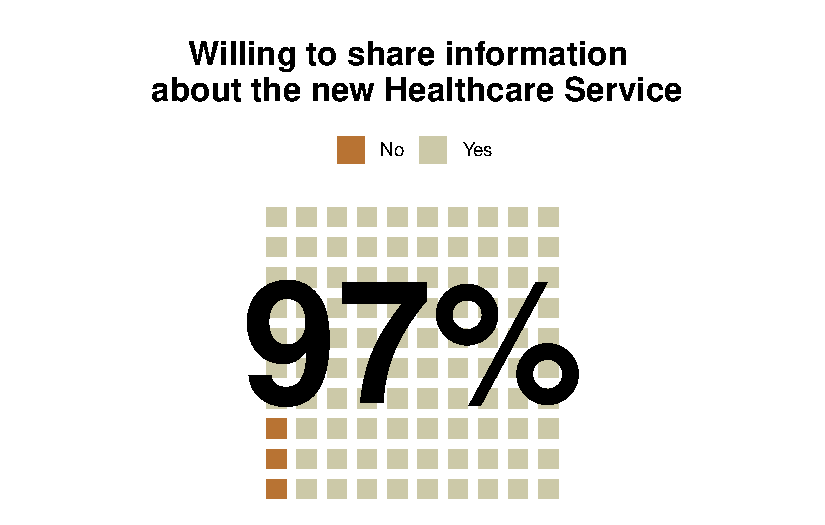
\includegraphics[keepaspectratio]{Utano_report_files/figure-pdf/unnamed-chunk-29-1.pdf}}

Approximately three in five individuals expressed willingness to serve
as community agents and earn an incentive by referring clients to the
new healthcare service. This indicates a strong opportunity to leverage
grassroots engagement as a powerful marketing and outreach channel.

\pandocbounded{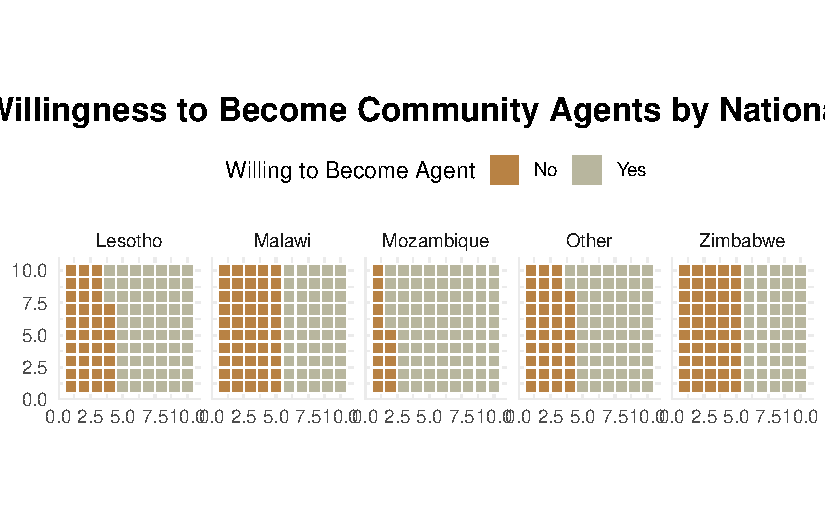
\includegraphics[keepaspectratio]{Utano_report_files/figure-pdf/unnamed-chunk-30-1.pdf}}

Notably, analysis of respondents' willingness to become community agents
for an incentive shows interesting relationship between perceived
package prestige and engagement interest. A higher proportion of
individuals enrolled in the mid-tier Gold (Yes - 62\%) and Silver (Yes -
73\%) health service packages expressed willingness to serve as
community agents compared to those who selected the more premium
Platinum (Yes - 48\%) and top-tier Lithium (Yes - 56\%) packages. This
suggests that individuals opting for less expensive packages may view
the community agent role as an opportunity to derive added value. In
contrast, those in higher-tier plans may have less motivation to engage
at a grassroots level.

The average commission rate across the total respondent population was
R1,596.16 per person referred. However, this average masks substantial
variation across nationality and gender subgroups. The reported
commission values ranged from a minimum of R2 to a maximum of R150,000,
indicating a highly skewed distribution.

When disaggregated by nationality, respondents from Lesotho reported the
highest average commission at R6,120---nearly four times the overall
average---suggesting a stronger perceived value or expectation for
referral incentives. Zimbabwe followed with a mean of R1,391, closely
aligning with the overall average. Respondents classified under `Other
nationalities' had a mean of R878, while Malawians and Mozambicans
reported significantly lower average commissions at R153 and R137,
respectively. This widespread view may reflect differences in economic
expectations, market exposure, or perceived effort-to-reward ratios
across national groups.

Gender-based analysis revealed that women, on average, expected
significantly higher commissions (R3,030) than their male and ``other
gender''counterparts, whose average responses ranged from R460 to R800.
This disparity may reflect differing motivations or opportunity costs
associated with participation in referral-based models.

Nearly half of the respondents (49\%) indicated that no formal
endorsement is needed, suggesting a high level of direct trust in the
service itself. About 34\% of respondents expressed a preference for
endorsement by their own government, indicating that messaging that
resonates with national identity and local credibility may be effective
for this group. Conversely, endorsements from private companies (18\%)
and the South African government (19\%) received the least support.

\pandocbounded{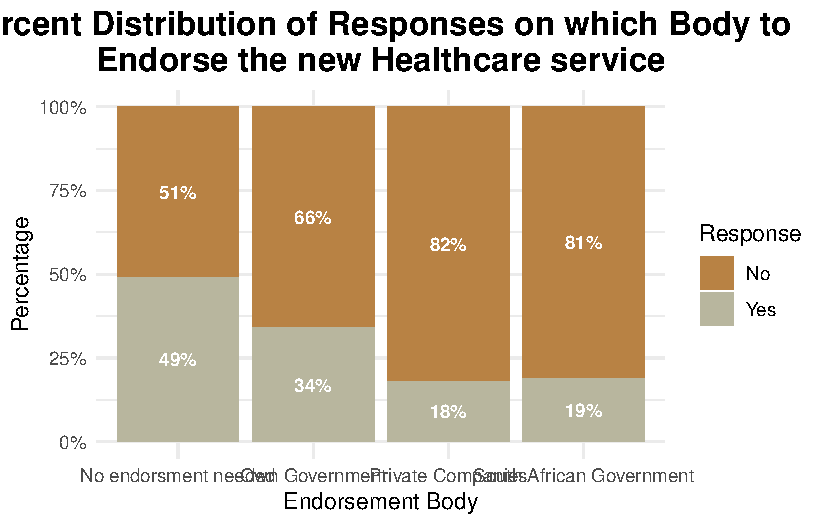
\includegraphics[keepaspectratio]{Utano_report_files/figure-pdf/unnamed-chunk-32-1.pdf}}




\end{document}
